\let\texyear\year
\documentclass{ieeeaccess}
\let\ieeeaccessyear\year
\let\year\texyear

\usepackage{cite}
\usepackage{amsmath,amssymb,amsfonts,mathtools}
\usepackage{amsthm}
\usepackage{algorithmic}
\usepackage{graphicx}
\usepackage{textcomp}
\usepackage{booktabs}
\usepackage{array}
\usepackage{enumitem}
\usepackage{xcolor}
\usepackage{url}
\usepackage{xspace}
\usepackage{comment}
\usepackage{tikz}
\usepackage{float}
\usepackage[caption=false]{subfig}
\usepackage{expl3}
\usepackage{xparse}
\usetikzlibrary{arrows.meta,shapes,automata,positioning,calc,fit,tikzmark,decorations.pathreplacing,decorations.markings}
% Unified monochrome figure style for the paper.
% All automata and timing diagrams use white states, black borders and black arrows.
\tikzset{
  fmstate/.style={
    circle, draw=black, fill=white, line width=0.6pt,
    minimum size=9mm, inner sep=1pt, font=\small
  },
  fmstatewide/.style={
    rounded rectangle, draw=black, fill=white, line width=0.6pt,
    minimum height=8mm, inner xsep=3pt, inner ysep=1.5pt, font=\small
  },
  fmaccept/.style={fmstate,double,double distance=1.2pt},
  fmerror/.style={fmstate,double,double distance=1.2pt,fill=gray!12},
  fmedge/.style={->,>=Stealth,line width=0.6pt},
  fmlabel/.style={font=\scriptsize,align=center,fill=white,inner sep=1.2pt},
  fminvariant/.style={font=\scriptsize,align=center},
  fmnote/.style={font=\scriptsize,align=center},
  fmtimeline/.style={->,>=Stealth,line width=0.6pt},
  fmevent/.style={circle,draw=black,fill=white,line width=0.6pt,minimum size=4.5mm,inner sep=0.5pt},
  fmreference/.style={fmevent,double,double distance=0.8pt},
  fmguide/.style={densely dashed,line width=0.45pt},
  fmbrace/.style={decorate,decoration={brace,amplitude=4pt},line width=0.5pt}
}


\providecommand{\Nat}{\mathbb{N}}
\providecommand{\Real}{\mathbb{R}}
\providecommand{\CVal}{\mathsf{val}}
\providecommand{\Val}{\mathsf{val}}
\providecommand{\Inv}{\mathit{Inv}}
\providecommand{\T}{\mathcal{T}}
\providecommand{\hEventually}{\widehat{\Diamond}}
\providecommand{\hAlways}{\widehat{\Box}}
\providecommand{\optimize}{\mathsf{optimize}}
\providecommand{\export}{\mathsf{export}}
\newtheorem{theorem}{Theorem}[section]
\newtheorem{lemma}[theorem]{Lemma}
\newtheorem{proposition}[theorem]{Proposition}
\newtheorem{corollary}[theorem]{Corollary}
\newtheorem{assumption}[theorem]{Assumption}
\newtheorem{definition}[theorem]{Definition}
\bibliographystyle{IEEEtran}
\let\year\ieeeaccessyear

\begin{document}
\history{}
\doi{}

\title{Mechanically Verified Optimization and UPPAAL Export for Timed B\"uchi Automata}
\author{\uppercase{Elie Fares}\authorrefmark{1},
\uppercase{Jean-Paul Bodeveix}\authorrefmark{2},
\uppercase{Hussain Al-Aqrabi}\authorrefmark{1} AND
\uppercase{Azar Salami}\authorrefmark{1}}
\address[1]{Higher Colleges of Technology\\Sharjah, United Arab Emirates\\(e-mail: efares@hct.ac.ae, halaqrabi@hct.ac.ae, asalami@hct.ac.ae)}
\address[2]{IRIT, UPS, Universit\'e de Toulouse, France (e-mail: bodeveix@irit.fr)}

\begin{abstract}
Timed B\"uchi automata (TBAs) produced by translators or supplied by other tools can contain redundant timing constraints, resets, transitions, clocks, and states, and may use disjunctive invariants that are unsuitable for direct UPPAAL export. We present a pipeline mechanically verified in Rocq (formerly Coq) that synthesizes location invariants, propagates timing bounds, removes infeasible transitions and dead resets, merges synchronously reset clocks and equivalent transitions and locations, and converts the result to conjunctive guards and invariants. Every pass preserves the timed-word language of every input TBA under the development's existential initial-clock semantics. In particular, the optimization theorem is generic in the automaton and in the number of rounds; the export theorem composes the verified transformations into a UPPAAL-oriented representation. The transformations are extracted to OCaml and used in \texttt{mtl2tba}. We report measurements on 31 automata generated from a fixed Metric Temporal Logic (MTL) benchmark, plus UPPAAL case studies. The data show large transition reductions on several inputs, while export can increase the edge count when it removes disjunctive invariants. These experiments evaluate the end-to-end tool on the benchmark automata; they do not measure a broad corpus of arbitrary TBAs.
\end{abstract}
\begin{keywords}
Rocq/Coq, formal verification, program extraction, timed automata, timed B\"uchi automata, UPPAAL, verified optimization.
\end{keywords}
\titlepgskip=-15pt
\maketitle

\section{Introduction}
\label{sec:introduction}
Timed B\"uchi automata are a common intermediate representation for real-time requirements and are also used as inputs to timed-language analysis tools. An automaton that is correct at the language level may still be inconvenient for downstream verification: its transition guards can repeat constraints, some resets may never affect a future guard, multiple clocks may evolve in lockstep, and the same behavior may be represented by many transitions. In addition, merging transitions can produce disjunctive guards and invariants, while UPPAAL-oriented automata are most useful with conjunctive guards and conjunctive upper-bound invariants.

An optimization pass is safe only when it preserves accepted timed words, including the treatment of clock resets, event labels, and B\"uchi acceptance. Several passes also interact. Propagating a lower bound may make a transition contradictory, but a synthetic nonnegativity guard can keep an otherwise dead clock live unless guards are normalized before reset analysis. Splitting a disjunctive invariant into copies also requires a condition on entry: choosing a copy whose invariant admits less time than another copy can change the accepted language.

This paper presents a mechanically verified post-processing and export pipeline for TBAs. Its central results quantify over an arbitrary input TBA, rather than only automata generated from a particular temporal logic. In Coq, we prove that each optimization and export operation preserves the automaton's timed-word language under the acceptance semantics formalized in the development. The optimizer theorem holds for every finite number of rounds, so the implementation can stop after reaching a structural fixed point or after its configured iteration bound without relying on convergence for correctness.

The transformations have two stages. The optimization stage synthesizes upper-bound location invariants, propagates target invariants backward into guards, propagates entry lower bounds forward, removes contradictory and unreachable transitions, removes dead resets, merges clocks reset synchronously, tightens guards, and merges transitions and locations. The export stage merges transitions with equal source, target, label, and resets; eliminates disjunctive invariants by creating copies with conjunctive invariants and clock-difference entry conditions; splits disjunctive guards; normalizes the result; and emits symbolic transitions for drawing.

The verified transformations are extracted to OCaml and used by \texttt{mtl2tba}. That tool includes an upstream MTL-to-TBA construction and an interface to Spot, but the preservation theorems in this paper apply to every TBA passed to the verified post-processing functions. The experiments use automata from 31 fixed MTL benchmark configurations, not a diverse arbitrary-TBA corpus. We therefore distinguish the universal proof claims from the benchmark-specific performance measurements.

The contributions are:
\begin{itemize}[leftmargin=*]
  \item a Coq development of language-preserving TBA transformations, including invariant synthesis and propagation, clock and state simplification, transition merging, and disjunctive-invariant elimination;
  \item a generic theorem for every TBA and every number of optimization rounds, plus a verified export composition whose final guards and invariants are conjunctive;
  \item an extracted implementation and an explicit account of its interface and trust boundaries; and
  \item a reproducible evaluation on the tracked 31-configuration benchmark and four system-model case studies, with results and limitations reported from repository data.
\end{itemize}
The integrated tool reuses the same shared-clock Rocq MTL-to-TBA translation proof presented in the companion TSE manuscript as its upstream construction. This translation proof is a prerequisite and is not a new contribution of this paper. The new formal results here begin with generic TBA optimization and export, and apply to every TBA passed to the verified post-processing functions. End-to-end MTL correctness additionally composes with the upstream translation result and its LTL-to-Buchi backend contract.

\section{Timed Automata and the Preservation Contract}
\label{sec:model}
\subsection{Timed words and TBAs}
A timed word is an infinite sequence $w=(a_i,t_i)_{i\in\Nat}$, where $a_i$ is an event from a finite alphabet $\Sigma$, timestamps are strictly increasing, and time diverges: $\lim_{i\to\infty}t_i=+\infty$. For each position $i$, let $\delta_i=t_{i+1}-t_i$ be the time from event $i$ to the next event. A clock valuation maps a finite clock set $X$ to $\Real_{\ge0}$. Guards are finite conjunctions of event literals and clock comparisons $x\bowtie c$ for $\bowtie\in\{<,\le,=,\ge,>\}$; transitions also carry a set of clocks to reset.

A TBA is a tuple $\mathcal A=(L,\ell_0,X,E,\mathit{Acc})$, where $L$ is a finite location set, $\ell_0$ is the initial location, $X$ is the clock set, $E$ is a finite set of transitions $(\ell,\alpha,g,Z,\ell')$, $\alpha$ is an event condition, $g$ is a clock guard, $Z\subseteq X$ is a reset set, and $\mathit{Acc}\subseteq L$ is the set of B\"uchi-accepting locations. The starting automata in the verified optimization are represented without location invariants; synthesis adds them as a separate annotation. Exported invariants are conjunctions of upper bounds.

The Coq development interprets transitions over an extended timed word that records clock values and reset decisions. Here $v_i$ is the clock valuation at event $i$, and $Z_i$ records the clocks reset by the transition on that event. Since a reset occurs at $t_i$, the next-event valuation includes the elapsed interval $\delta_i$:
\[
v_{i+1}(x)=
\begin{cases}
\delta_i,&x\in Z_i,\\
v_i(x)+\delta_i,&x\notin Z_i.
\end{cases}
\]
A run chooses one enabled transition per position and visits accepting locations infinitely often. The accepted language existentially quantifies over clock-consistent extensions of the base timed word, including the initial clock values. This is the acceptance notion of the generic preservation theorems; conventional initialization at zero is a separate deployment concern.

For an annotated automaton, an invariant must hold throughout the delay spent at its location. Since synthesized invariants are conjunctions of non-strict upper bounds and clocks are nondecreasing during a delay, holding at the event at the end of the delay is equivalent to holding throughout that stay. The proof formalizes this trace-model equivalence and uses it to show that the annotations and strengthening operations preserve timed words.

\subsection{What export must preserve}
\label{sec:export-contract}
The export must retain the same transition alphabet, B\"uchi marking, clock meaning, and timed-word language. It may change the number of locations, transitions, and clocks, and may introduce difference constraints in transition guards to choose among invariant copies. Such choices must not create or delete an accepted timed word. The target representation has conjunctive guards and conjunctive location invariants; a later symbolic representation groups transitions with identical source, target, and reset sets under Boolean labels.

All main preservation theorems below are stated for arbitrary input TBAs. Their proof does not require properties of the MTL translation or Spot. An upstream correctness theorem can be composed with these results, but Spot's correctness and the soundness of the front end are outside the generic pass theorems.

\section{Verified Optimization}
\label{sec:post}
After invariant synthesis, the optimization pipeline alternates timing propagation with simplification. Synthesized upper bounds expose how long an automaton can remain at a location. Propagating them to incoming guards can make lower and upper constraints jointly inconsistent; forward propagation supplies complementary lower-bound information. The pipeline then removes transitions, resets, clocks, and duplicate structure that no longer affect the language.

\begin{table*}[t]
\centering
\caption{Verified post-processing passes. Each preservation theorem quantifies over every input TBA under the Coq timed-word semantics. Detailed definitions and proof arguments follow in this section.}
\label{tab:post-passes}
\small
\begin{tabular}{@{}p{0.42\textwidth}p{0.52\textwidth}@{}}
\toprule
Pass & Coq preservation theorem\\
\midrule
Upper-bound invariant synthesis & \texttt{add\_invariants\_accepts}\\
Backward propagation ($n$ steps) & \texttt{propagate\_n\_accepts}\\
Forward propagation of lower bounds & \texttt{forward\_accepts}\\
Two-sided invariants & \texttt{add\_two\_sided\_invariants\_accepts}\\
Removal of contradictory transitions & \texttt{remove\_contradictory\_accepts}\\
Removal of locations without entering transitions & \texttt{remove\_unreachable\_accepts}\\
Removal of dead resets & \texttt{remove\_dead\_resets\_accepts}\\
Merging synchronously reset clocks & \texttt{merge\_all\_accepts}\\
Normalization of guards & \texttt{normalize\_accepts}\\
Removal of unsatisfiable action labels & \texttt{remove\_unsat\_accepts}\\
Merging transitions & \texttt{merge\_trans\_accepts}\\
Merging equivalent locations & \texttt{merge\_states\_all\_accepts}\\
Iterated pipeline ($n$ rounds) & \texttt{optimize\_accepts}\\
Merging transitions for export & \texttt{merge\_transitions\_accepts}\\
Elimination of disjunctive invariants & \texttt{split\_accepts}\\
Splitting of disjunctive guards & \texttt{explode\_accepts}\\
Normalization of exported guards & \texttt{normalize\_d\_accepts}\\
Removal of copies never entered & \texttt{dprune\_n\_accepts}\\
Merging of the initial location & \texttt{dmerge\_states\_all\_accepts}\\
Symbolic transitions & \texttt{symbolic\_ext\_accepts}\\
Complete export & \texttt{export\_accepts}\\
\bottomrule
\end{tabular}
\end{table*}

\begin{figure}[t]
\centering
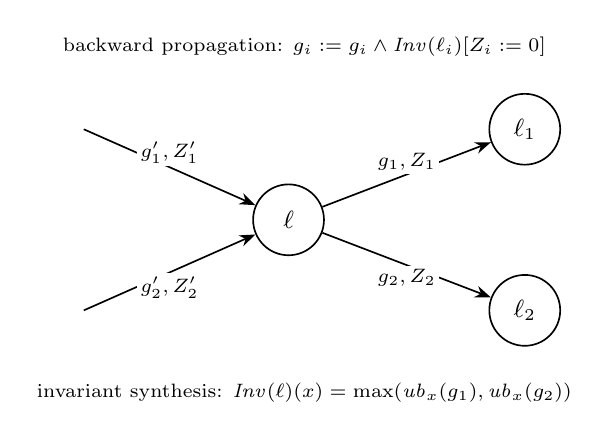
\begin{tikzpicture}[node distance=20mm]
  \node[fmstate] (L) at (0,0) {$\ell$};
  \node[fmstate] (S1) at (3.0,1.15) {$\ell_1$};
  \node[fmstate] (S2) at (3.0,-1.15) {$\ell_2$};
  \coordinate (P1) at (-2.6,1.15);
  \coordinate (P2) at (-2.6,-1.15);
  \draw[fmedge] (P1) -- node[fmlabel,above] {$g'_1,Z'_1$} (L);
  \draw[fmedge] (P2) -- node[fmlabel,below] {$g'_2,Z'_2$} (L);
  \draw[fmedge] (L) -- node[fmlabel,above] {$g_1,Z_1$} (S1);
  \draw[fmedge] (L) -- node[fmlabel,below] {$g_2,Z_2$} (S2);
  \node[fmnote] at (0.20,2.20) {backward propagation: $g_i:=g_i\land \mathit{Inv}(\ell_i)[Z_i:=0]$};
  \node[fmnote] at (0.20,-2.20) {invariant synthesis: $\mathit{Inv}(\ell)(x)=\max(\mathit{ub}_x(g_1),\mathit{ub}_x(g_2))$};
\end{tikzpicture}

\caption{Invariant computation. Successor invariants strengthen outgoing
guards; upper bounds of the resulting guards resynthesize the source
invariant. Reset sets determine which target-clock constraints become
constant.}
\label{fig:main-inv-unified}
\end{figure}

\subsection{Location Invariants on the Trace Model}
\label{sec:inv-semantics}
A location invariant maps every clock $x$ either to an upper bound
$M\in\mathbb R$, standing for the constraint $x\le M$, or to $+\infty$ (no
constraint).  We interpret automata with invariants on the extended words of
Section~\ref{sec:model}, as we do for automata without invariants.
Along a run $r$, the automaton stays in location $r(i)$ between the events
$i-1$ and $i$, and the invariant of $r(i)$ must hold during the whole stay,
that is, at the clock values $\CVal_\rho(i,x)-\tau$ for every delay
$\tau\in[0,\Delta_{i-1}]$, where $\Delta_{i-1}=t_i-t_{i-1}$ (and at the values $\CVal_\rho(0,x)$ for the
initial location).  This is the condition of Section~\ref{sec:model}, read at
the event that ends the stay.  Since clocks increase while time elapses, an
invariant made of upper bounds holds during the stay if and only if it holds at
the event that ends it (lemma \texttt{inv\_\allowbreak{}during\_\allowbreak{}iff\_\allowbreak{}at\_\allowbreak{}event}).
For the two-sided invariants of Section~\ref{sec:forward}, a lower bound
$x\ge m$ must likewise hold during the whole stay, hence at its beginning.

\subsection{Invariant Synthesis and Backward Propagation}
\label{sec:uppaal-invariants}\label{sec:main-invariants}
In the exported timed automaton, upper-bounded guards need invariants so that
time does not elapse past all useful outgoing transitions.  We compute location
invariants from outgoing upper bounds and propagate successor requirements
backward, following the standard timed-automata intuition of propagating
admissible time domains~\cite{[BGD04]}.

\paragraph{Upper bound of a guard.}
For a conjunctive guard $g$ and a clock $x$, let $\mathit{ub}_x(g)$ be the
smallest bound $m$ of the constraints $x\le m$, $x<m$, and $x=m$ occurring in
$g$, and $+\infty$ if $g$ contains none.  Other constraints are ignored.  A
valuation satisfying $g$ satisfies $x\le\mathit{ub}_x(g)$.

\paragraph{Invariant synthesis.}
For a location $\ell$ with outgoing transitions
$\ell\xrightarrow{g_i,Z_i}\ell_i$, $i=1,\dots,m$, the synthesized invariant is
\[
  \mathit{Inv}(\ell)(x)=\max_{1\le i\le m}\mathit{ub}_x(g_i),
\]
with $\mathit{Inv}(\ell)(x)=+\infty$ when $\ell$ has no outgoing transition.
Thus a clock that some outgoing guard does not bound does not appear in the
invariant.  The bound is always non-strict, even when it comes from a strict
guard $x<m$: the invariant only needs to be implied by the guard of the next
transition, and strictness is kept in the guards themselves.

\begin{theorem}[Invariant synthesis]
\label{thm:inv-synthesis}
For every TBA $\mathcal A$, the automaton $\mathcal A$ with the synthesized
invariants accepts the same timed words as $\mathcal A$.
\end{theorem}

\begin{proof}
Adding invariants can only remove runs.  Conversely, let $r$ be an accepting
run on $\rho$.  At every event $i$, the transition taken from $r(i)$ is enabled,
so its guard holds at the values $\CVal_\rho(i,x)$, which are therefore at most
$\mathit{Inv}(r(i))(x)$.  By the lemma \texttt{inv\_\allowbreak{}during\_\allowbreak{}iff\_\allowbreak{}at\_\allowbreak{}event}, the invariant of $r(i)$ holds during
the whole stay.  (Coq: \texttt{add\_\allowbreak{}invariants\_\allowbreak{}correct}.)
\end{proof}

\paragraph{Backward propagation.}
One propagation step strengthens every transition
$\ell\xrightarrow{g,Z}\ell'$ with the invariant of its target after the
resets:
\[
  g := g\wedge\mathit{Inv}(\ell')[Z:=0],
\]
where $\mathit{Inv}(\ell')[Z:=0]$ replaces every bound $x\le M$ on a reset clock
$x\in Z$ by the constant constraint $0\le M$, that is, by $\top$ if $M\ge0$ and
by $\bot$ otherwise.  Invariants are then synthesized again from the
strengthened guards.

\begin{theorem}[Backward propagation]
\label{thm:propagation}
For every TBA $\mathcal A$ and every $n\in\mathbb N$, the automaton obtained by
$n$ propagation steps accepts the same timed words as $\mathcal A$.
\end{theorem}

\begin{proof}
Strengthening guards can only remove runs.  Conversely, consider an accepting
run that takes $\ell\xrightarrow{g,Z}\ell'$ at event $i$ and then a transition
$\ell'\xrightarrow{g',Z'}\ell''$ at event $i+1$.  The second guard holds at event
$i+1$, so the values at that event are bounded by $\mathit{Inv}(\ell')$.  Clock
consistency gives $\CVal_\rho(i+1,x)=\Delta_i$ for $x\in Z$ and
$\CVal_\rho(i+1,x)=\CVal_\rho(i,x)+\Delta_i\ge\CVal_\rho(i,x)$ otherwise; hence
the strengthened guard $g\wedge\mathit{Inv}(\ell')[Z:=0]$ holds at event $i$.
The argument uses clock consistency, so the theorem is stated on timed words.
(Coq: \texttt{propagate\_\allowbreak{}accepts} and
\texttt{propagate\_\allowbreak{}n\_\allowbreak{}accepts}.)
\end{proof}

Each round of the optimization pipeline of Section~\ref{sec:main-pipeline}
applies one propagation step.  The tool repeats the rounds until the
automaton is structurally equal to the previous one, as an OCaml value, or
until 50 rounds have been performed; the bound guarantees termination, and the
theorem holds for every number of steps, whether or not a fixpoint is
reached.  On our benchmarks, the rounds reach a fixpoint after at most five
rounds.
The invariant computation at one location is summarized in the article's
Figure~\ref{fig:main-inv-unified}.

\paragraph{Example.}
We illustrate the algorithm on the automaton of Fig.~\ref{fig:inv-example},
which contains a two-location cycle $\ell_1\to\ell_2\to\ell_1$ and a self-loop
at $\ell_2$.  It has one clock $x$, the initial location $\ell_0$, and the
transitions
\[
\begin{aligned}
&\ell_0 \xrightarrow{a,\;Z=\{x\}} \ell_1,\quad
 \ell_1 \xrightarrow{b,\;x\le 2,\;Z=\emptyset} \ell_2,\\
&\ell_2 \xrightarrow{c,\;\top,\;Z=\emptyset} \ell_1,\quad
 \ell_2 \xrightarrow{d,\;x\le 1,\;Z=\emptyset} \ell_2.
\end{aligned}
\]
The edge $\ell_1\xrightarrow{b}\ell_2$ requires $x\le2$, and the self-loop at
$\ell_2$ requires the tighter bound $x\le1$.

\begin{figure}[t]
\centering
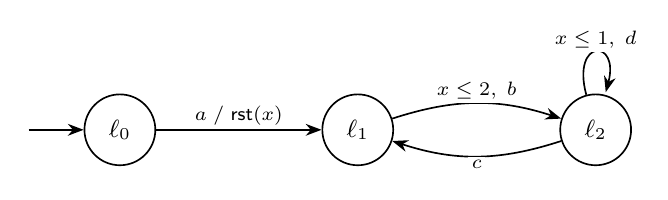
\begin{tikzpicture}[node distance=21mm]
  \node[fmstate] (l0) {$\ell_0$};
  \node[fmstate,right=of l0] (l1) {$\ell_1$};
  \node[fmstate,right=of l1] (l2) {$\ell_2$};
  \draw[fmedge] ([xshift=-7mm]l0.west) -- (l0.west);
  \draw[fmedge] (l0) -- node[fmlabel,above] {$a\;/\;\mathsf{rst}(x)$} (l1);
  \draw[fmedge] (l1) to[bend left=18] node[fmlabel,above] {$x\le2,\;b$} (l2);
  \draw[fmedge] (l2) to[bend left=18] node[fmlabel,below] {$c$} (l1);
  \draw[fmedge] (l2) edge[loop above] node[fmlabel] {$x\le1,\;d$} (l2);
\end{tikzpicture}

\caption{Automaton used to illustrate invariant propagation, with one clock $x$
and actions $a$--$d$.  Edges are labeled ``guard, action / resets'' (the guard
is omitted when it is $\top$); only the edge $\ell_0\to\ell_1$ resets $x$.  The
incoming arrow marks the initial location; acceptance plays no role here.  The
computed fixpoint is $\mathit{Inv}(\ell_1)=\mathit{Inv}(\ell_2)=(x\le2)$.}
\label{fig:inv-example}
\end{figure}

\begin{enumerate}
\item \emph{Synthesis.}  $\mathit{Inv}(\ell_1)(x)=\mathit{ub}_x(x\le2)=2$.  At
$\ell_2$, $\mathit{Inv}(\ell_2)(x)=\max(1,+\infty)=+\infty$, because the
transition toward $\ell_1$ does not bound $x$.  At $\ell_0$, the only outgoing
guard is $\top$, so $\mathit{Inv}(\ell_0)(x)=+\infty$.

\item \emph{Propagation.}  The transition
$\ell_2\xrightarrow{c,\;Z=\emptyset}\ell_1$ becomes guarded by
$\top\wedge\mathit{Inv}(\ell_1)=(x\le2)$.  The transition
$\ell_0\xrightarrow{a,\;Z=\{x\}}\ell_1$ receives $(0\le2)\equiv\top$ and is
unchanged.

\item \emph{Synthesis.}  At $\ell_2$, the outgoing guards are now $x\le1$ and
$x\le2$, so $\mathit{Inv}(\ell_2)(x)=\max(1,2)=2$.

\item \emph{Propagation.}  The transition $\ell_1\xrightarrow{b,\;x\le2}\ell_2$
receives $x\le2$, which it already contains, and the self-loop at $\ell_2$
receives $x\le2$, which is implied by $x\le1$.  Nothing changes.
\end{enumerate}
The fixpoint is $\mathit{Inv}(\ell_0)=\top$ and
$\mathit{Inv}(\ell_1)=\mathit{Inv}(\ell_2)=(x\le2)$.  While the automaton
remains in the cycle $\ell_1\leftrightarrow\ell_2$, the clock $x$ cannot exceed
$2$, and at every reachable valuation at least one outgoing transition of the
current location is enabled.  The invariants do not remove every blocking
behavior: since $x$ is never reset in the cycle, time is blocked once $x=2$.
They make the upper bounds of the property automaton explicit, and
Theorems~\ref{thm:inv-synthesis} and~\ref{thm:propagation} guarantee that they
do not change its language.

\subsection{Forward Propagation of Lower Bounds and Simplification}
\label{sec:forward}\label{sec:main-forward}
\paragraph{Entry bounds.}
Dually, for a transition $t=\ell\xrightarrow{g,Z}\ell'$ and a clock $x$, the
\emph{entry bound} of $x$ along $t$ is $0$ if $x\in Z$ and otherwise the
largest bound $\mathit{lb}_x(g)$ of the constraints $x\ge m$, $x>m$, and $x=m$
of $g$, if any.  The entry bound of $x$ at a location $\ell'$ is the minimum of
the entry bounds of $x$ along the transitions entering $\ell'$; for the initial
location, the initial entry, with bound $0$, also counts.  If some entering
transition gives no bound on $x$, the clock $x$ has no entry bound at $\ell'$.
Since clocks are nonnegative and do not decrease while time elapses, every
clock with entry bound $m$ at $\ell'$ satisfies $x\ge m$ during every stay in
$\ell'$.

\paragraph{Forward propagation.}
The forward step adds $x\ge m$ to the guard of every transition leaving
$\ell'$, for every clock $x$ with entry bound $m$ at $\ell'$ (Coq:
\texttt{forward\_\allowbreak{}accepts}).  The entry bounds can also be read as lower-bound
invariants: the two-sided automaton that carries the synthesized upper-bound
invariants and the entry bounds as lower-bound invariants accepts the same
timed words (\texttt{add\_\allowbreak{}two\_\allowbreak{}sided\_\allowbreak{}invariants\_\allowbreak{}accepts}).  UPPAAL
rejects lower-bound invariants, and their only role is to make infeasible
transitions visible: after forward and backward propagation, a transition whose
source location bounds a clock from below and whose target bounds it from above
carries both bounds in its guard.

\paragraph{Simplification.}
Three simplifications follow.  First, a transition whose guard contains
contradictory constraints is removed: a lower bound and an upper bound on the
same clock with $u<l$, or with $u=l$ and one of them strict, or an upper bound
$x\le u$ with $u<0$ or $x<u$ with $u\le0$.  Such a transition is never enabled (Coq:
\texttt{remove\_\allowbreak{}contradictory\_\allowbreak{}accepts}).  Second, the transitions
leaving a non-initial location that has no entering transition
are removed: such a location never occurs on a run after position~$0$ (Coq:
\texttt{remove\_\allowbreak{}unreachable\_\allowbreak{}accepts}).  The iteration of the pipeline
removes chains of such locations one step at a time.  A location whose only
entering transitions are self-loops keeps them, but it is unreachable from
the initial location; the tool counts and prints only the locations
reachable from the initial one and their transitions.  Third, a transition whose
action label is unsatisfiable, because it requires two different actions or an
action and its negation, is removed (Coq:
\texttt{remove\_\allowbreak{}unsat\_\allowbreak{}accepts}).  Such labels arise because the
translator treats an action $a$ and the atom $\neg a$ of $\T(f)$ as independent
propositions; removing them also enables clock merging, since the resets of a
transition that can never be taken would otherwise prevent it.

\subsection{Dead Resets and Merging of Synchronously Reset Clocks}
\label{sec:dead-merge}\label{sec:main-dead-merge}
\paragraph{Dead resets.}
A clock $x$ is \emph{live} at a location $\ell$ if some transition that tests
$x$ in its guard can be taken from $\ell$, possibly after other transitions.
The live locations are computed as a backward closure, along all
transitions, from the sources of the transitions that test $x$; the other
locations are \emph{dead} for $x$.  Since the correctness of the pass does
not depend on how this closure is computed, the pass checks the two
properties that the proof uses, namely that no transition leads from a dead
location to a live one and that none tests $x$ from a dead location, and then removes $x$ from the reset sets of the
transitions that enter a dead location.  After such a transition, the value of
$x$ is never read again, so whether it is reset does not matter.  The proof
builds, from every accepted extended word, an extended word that differs only
in the reset decisions of $x$, and conversely (Coq:
\texttt{remove\_\allowbreak{}dead\_\allowbreak{}resets\_\allowbreak{}clock\_\allowbreak{}accepts}).  The pass is applied
to every clock (\texttt{remove\_\allowbreak{}dead\_\allowbreak{}resets\_\allowbreak{}accepts}).

\paragraph{Synchronous clocks.}
The verified translation shares the clock of syntactically identical timed
subformulas.  Clocks of \emph{different} subformulas can also be merged when
they are reset synchronously.  Two clocks $x\neq y$ are \emph{mergeable} if
\begin{enumerate}[label=(\roman*)]
  \item every transition resets $x$ if and only if it resets $y$;
  \item no transition enters the initial location; and
  \item every transition leaving the initial location resets $x$ and does not
        test it.
\end{enumerate}
Then, after the first event, $x$ and $y$ always have the same value, and every
test of $x$ can be replaced by the same test on $y$ (Coq:
\texttt{merge\_\allowbreak{}accepts}).  The condition is checked by a Boolean function
proved to imply it, and the pass tries all pairs of reset clocks
(\texttt{merge\_\allowbreak{}all\_\allowbreak{}accepts}).  The merged clock $x$ is no longer tested,
so its remaining resets are removed by the dead-reset pass in the next round.
This verified merging is restricted to synchronously reset clocks; merging
clocks whose values coincide for other reasons is not covered.

\subsection{Normalization of Guards}
\label{sec:normalize}
Backward and forward propagation add constraints to guards.  Every time a
guard is strengthened, it is \emph{tightened}: a constraint implied by another
constraint of the same guard on the same clock is dropped, so that a guard
keeps at most one lower bound and one upper bound per clock (an equality
counting as both); for instance, $x\le5\land x<2$ becomes $x<2$.  The
implication test compares bounds and strictness, and is proved sound (Coq:
\texttt{tighten\_\allowbreak{}holds}).  Normalization tightens every guard and also
removes the lower bounds $x\ge m$ with $m\le0$ and $x>m$ with $m<0$, which every
clock value satisfies; it is needed after the merging of clocks, which renames
constraints.  The removal of trivial lower bounds relies on the nonnegativity
of clock values, so the theorem is stated on timed words (Coq:
\texttt{normalize\_\allowbreak{}accepts}).

\subsection{Merging of Transitions and of Locations}
\label{sec:merge-ts}\label{sec:main-merge-ts}
\paragraph{Transitions.}
Two transitions with the same source, target, and resets are merged when the
union of their enabling conditions is again a conjunction.  A transition is
removed when another transition with the same source, target, and resets is
\emph{weaker}, that is, when its label and guard imply those of the other
transition, constraint by constraint (subsumption).  Two transitions
whose labels, or guards, differ only by a literal and its negation, such as
$p$ and $\neg p$, $x<2$ and $x\ge2$, or $x\le5$ and $x>5$, are replaced by one
transition without that literal (resolution).  The pass preserves the language
because every enabled transition has an enabled counterpart with the same
source and target, and conversely (Coq: \texttt{merge\_\allowbreak{}trans\_\allowbreak{}accepts}).
The other unions are disjunctive; they are formed by the export
(Section~\ref{subsec:disjunctive-invariants}).

\paragraph{Locations.}
A location $\ell'$ is merged into a location $\ell$ when both are accepting or
both are not, and when every transition leaving $\ell'$ has a twin leaving
$\ell$, and conversely: same label, guard, and resets, compared as sets, and
same target once $\ell'$ is replaced by $\ell$.  The transitions entering
$\ell'$ are redirected to $\ell$, and those leaving $\ell'$ are removed.  A run
of the original automaton becomes a run of the merged one by replacing $\ell'$
by $\ell$; conversely, a run of the merged automaton is followed in the
original one, taking in $\ell'$ the twin of the transition taken in $\ell$
(Coq: \texttt{merge\_\allowbreak{}states\_\allowbreak{}all\_\allowbreak{}accepts}; ``state'' in a Coq name
means location).  The condition on the B\"uchi marking is necessary: merging
an accepting location with a non-accepting twin would accept runs that visit only the latter infinitely
often.


\subsection{Transition Merging and Elimination of Disjunctive Invariants}
\label{subsec:disjunctive-invariants}

The export works on a model whose guards are in disjunctive normal form over
clock constraints and clock-difference constraints $x-y\le b$, and whose
location invariants are disjunctions of conjunctions of upper bounds.  It is
interpreted on the same trace model as before.  The export merges
transitions, splits locations, splits disjunctive guards, normalizes the
result, and merges the initial location with an equivalent one, each pass
being proved to preserve the language of timed words; it
ends with an
automaton whose guards and invariants are conjunctive, as UPPAAL requires
(Coq: \texttt{export\_\allowbreak{}accepts},
\texttt{export\_\allowbreak{}guards\_\allowbreak{}conjunctive}, and
\texttt{export\_\allowbreak{}invariants\_\allowbreak{}conjunctive}).

\paragraph{Transition merging.}
Transitions with the same source, target, action label, and reset set are
merged into one transition whose guard is the disjunction of their guards (Coq:
\texttt{merge\_\allowbreak{}transitions\_\allowbreak{}accepts}).  The invariant of a location
$\ell$ is then naturally disjunctive: it has one disjunct
$\mathit{ub}(g)$, the conjunction of the upper bounds of $g$, for every
conjunct $g$ of every guard leaving $\ell$:
\[
  I = I_1 \lor \cdots \lor I_r.
\]
A disjunct that implies another disjunct is redundant and is dropped.  The
resulting invariant is more precise than the clock-by-clock maximum of
Section~\ref{sec:uppaal-invariants}, which is its conjunctive
over-approximation.

\paragraph{Splitting locations.}
UPPAAL does not allow disjunctive location invariants: invariants must be
conjunctions of clock constraints defining convex, past-closed zones.  A
location with invariant $I_1\lor\cdots\lor I_r$ is therefore replaced by
locations with conjunctive invariants and the same timed behavior.  Bodeveix
and Filali studied disjunctive invariants in UPPAAL~\cite{[BF03]}.
Figure~\ref{fig:disj-general} in the article summarizes the transformation.

The location $L$ is replaced by one copy $L_k$ for each disjunct $I_k$, with
the conjunctive invariant $I_k$.  Every transition entering $L$ is replicated
toward every copy $L_k$, and its guard is strengthened with the entry condition
$\mathit{Ent}_k$ after the resets; every transition leaving $L$ is replicated from every
copy.  The disjunctive invariant itself is never built: the copies introduce
the conjunctive invariants directly, and the theorem compares the split
automaton with the automaton without invariants.  The run starts in a dedicated
copy of the initial location, without an invariant, since it is not entered by a
transition.  In the Coq development, the copy $k$ of location $\ell$ is numbered
$\ell\cdot\kappa+k$, where $\kappa-1$ is the largest number of disjuncts and the copy
$\kappa-1$ is the initial one; numbers that correspond to no disjunct are unreachable
locations.

\paragraph{Entry condition.}
The disjuncts need not be mutually exclusive, so simple replication would
introduce nondeterministic choices and could select a copy that permits less
time to elapse than another one.  The entry condition therefore selects a copy
with the \emph{longest} admissible delay.  The synthesized invariants have
non-strict bounds only (Section~\ref{sec:uppaal-invariants}); let
\[
  I_k = \bigwedge_{c\in C_k} c\le m^k_c.
\]
From a valuation $v$, $I_k$ admits the delays up to
$\mathit{Del}_k(v)=\min_{c\in C_k}(m^k_c-v(c))$, with $\mathit{Del}_k(v)=+\infty$ when $C_k$ is
empty.  The entry condition of $L_k$ requires $I_k$ and $\mathit{Del}_l(v)\le \mathit{Del}_k(v)$ for
every other copy $l$.  The comparison $\mathit{Del}_l\le \mathit{Del}_k$ holds when some bound
$c'\in C_l$ is reached no later than every bound $c\in C_k$, which is expressed
with clock differences:
\[
\mathit{Ent}_k\triangleq I_k \land
\bigwedge_{l\neq k}\ \bigvee_{c'\in C_l}\ \bigwedge_{c\in C_k}
 \bigl(c-c'\le m^k_c-m^l_{c'}\bigr).
\]
When $C_k$ is empty, the copy admits every delay and, since redundant
disjuncts are removed beforehand, no other $C_l$ is empty, so that the
conjunction over $l$ is true.  Ties are allowed: when two copies admit the same delay, both entry
conditions hold.

\begin{theorem}[Elimination of disjunctive invariants]
\label{thm:split}
The split automaton accepts the same timed words as the automaton without
invariants.
\end{theorem}

\begin{proof}
Every copy $L_k$ behaves as $L$ with additional constraints, so the split
automaton accepts no new word.  Conversely, consider an accepting run that
enters $L$ with the valuation $v$ (after the resets) and leaves it after a
delay $\tau$ along a transition whose guard has a conjunct $g$.  This
conjunct holds at $v+\tau$, hence so does the disjunct $\mathit{ub}(g)=I_j$,
and $\mathit{Del}_j(v)\ge\tau$.  If $I_j$ was dropped because it implies a kept disjunct, that disjunct admits
at least the same delays, so we may assume that $I_j$ is kept (Coq:
\texttt{disj\_\allowbreak{}inv\_\allowbreak{}cover}).  Choose a copy $k$ whose delay
$\mathit{Del}_k(v)$ is maximal (Coq: \texttt{best}).  Its entry condition holds at $v$, and
$\mathit{Del}_k(v)\ge \mathit{Del}_j(v)\ge\tau$,
so $I_k$ holds during the whole stay.  The successor copies are chosen in the
same way at every position.  Clock-difference constraints are invariant under
the elapse of time, so $\mathit{Ent}_k$ can be checked on the valuation after the resets,
and $\mathit{Ent}_k[Z:=0]$ on the valuation before them.  (Coq:
\texttt{split\_\allowbreak{}accepts}.)
\end{proof}

The substitution $[Z:=0]$ maps a difference $c-c'\le b$ to $0\le b$ when both
clocks are reset, to $c'\ge -b$ when only $c$ is reset, and to $c\le b$ when
only $c'$ is reset.  The disjunctions over $c'$ in $\mathit{Ent}_k$, and those created by
transition merging, are finally eliminated by putting the guards into
disjunctive normal form and splitting every transition into one copy per
disjunct (Coq: \texttt{explode\_\allowbreak{}accepts}).  In the worst case, the number
of copies is the product of the sizes of the disjunctions.

\paragraph{Final normalization.}
The guards are normalized before and after the split (Coq:
\texttt{normalize\_\allowbreak{}d\_\allowbreak{}accepts}): in every conjunction, constraints
implied by another one are removed, as in Section~\ref{sec:normalize}, together
with the trivial differences $x-x\le b$ with $b\ge0$; conjunctions containing a
difference $x-x\le b$ with $b<0$ are unsatisfiable and are removed; and a
conjunction that implies another conjunction of the same guard is removed.
Finally, the transitions leaving a location that is neither initial nor the
target of a transition are removed, until nothing changes (Coq:
\texttt{dprune\_\allowbreak{}n\_\allowbreak{}accepts}); this removes in particular the
transitions of the copies that correspond to no disjunct.  The dedicated copy
of the initial location is then merged into another location when both have
the same acceptance status, equivalent invariants (an invariant with an empty
disjunct being equivalent to no invariant), and the same outgoing
transitions, compared as sets after redirection; this is the case, for
instance, when the initial location has no invariant (Coq:
\texttt{dmerge\_\allowbreak{}states\_\allowbreak{}all\_\allowbreak{}accepts}).  The resulting
automaton has conjunctive guards with difference constraints and conjunctive
location invariants made of upper bounds.

\paragraph{Symbolic transitions.}
Each transition of the exported automaton reads a cube: a conjunction of
action literals and a conjunction of clock constraints.  For the drawing and
for the comparison with tools whose transitions carry Boolean formulas, the
last pass merges all the transitions with the same source, target, and
resets into one \emph{symbolic transition}, labeled by a disjunction of cases
$E_1\wedge c_1\vee\dots\vee E_k\wedge c_k$, where $E_j$ is a set of events,
either finite or the complement of a finite set, and $c_j$ a conjunction of
clock constraints; the cases with the same constraints are merged by union of
their sets of events.  A symbolic transition is enabled when the current
event belongs to some $E_j$ whose constraints $c_j$ hold, and its resets match
those of the extended word.  The symbolic automaton accepts the same extended
words as the exported one, hence the same timed words for both the
existential and the conventional acceptance (Coq:
\texttt{symbolic\_\allowbreak{}ext\_\allowbreak{}accepts},
\texttt{MTL\_\allowbreak{}to\_\allowbreak{}symbolic\_\allowbreak{}correct\_\allowbreak{}with}, and
\texttt{MTL\_\allowbreak{}to\_\allowbreak{}symbolic\_\allowbreak{}correct0\_\allowbreak{}with}).
The UPPAAL model keeps the conjunctive transitions, since a UPPAAL edge
synchronizes on one channel and its clock guard must be a conjunction.




\subsection{Iterated optimization}
\label{sec:main-pipeline}
In right-to-left function-composition order, one optimization round is
\[
\begin{aligned}
\mathsf{optimize\_step}={}&\mathsf{merge\_states}\\
 &\circ\mathsf{merge\_trans}\circ\mathsf{normalize}\\
 &\circ\mathsf{merge\_clocks}\circ\mathsf{dead\_resets}\\
 &\circ\mathsf{normalize}\circ\mathsf{unreachable}\\
 &\circ\mathsf{unsat\_labels}\circ\mathsf{contradictory}\\
 &\circ\mathsf{forward}\circ\mathsf{propagate}.
\end{aligned}
\]
The order is deliberate. Forward propagation can add $x\ge0$ after a reset;
the first normalization removes this tautology before dead-reset analysis,
which would otherwise treat the clock as live. Each operation may enable
later simplifications, so the driver repeats the round until the TBA is
structurally unchanged or 50 rounds have run. The theorem is independent of
this stopping rule and holds for every $n$.

\begin{theorem}[Optimization]
\label{thm:optimization}
For every TBA $\mathcal A$ and every $n\in\Nat$, $\optimize(n,\mathcal A)$ accepts exactly the timed words accepted by $\mathcal A$.
\end{theorem}
\begin{proof}
Every constituent operation preserves acceptance, as listed in Table~\ref{tab:post-passes}. Their composition preserves acceptance, and induction on $n$ proves the statement for every number of rounds. The mechanized result is \texttt{optimize\_accepts}.
\end{proof}

The extracted function also returns synthesized upper-bound invariants and entry bounds. The tool compares successive automata structurally and stops when they are equal or after 50 rounds. The theorem holds independently of whether iteration reaches a fixed point or uses all 50 rounds. In the tracked benchmark, observed rounds reach a fixed point within five rounds; this is a measured property of those inputs, not a termination assumption in the proof.

\section{UPPAAL-Oriented Export}
\label{sec:export}
The optimized automaton has normalized conjunctive guards. Export first merges transitions that agree on source, target, event label, and resets, placing their guards into a disjunction. The location invariant is then represented by disjunctions of conjunctions of upper bounds. UPPAAL-oriented output requires each such invariant to be conjunctive.

A location with invariant $I_1\lor\cdots\lor I_r$ is replaced by copies, one for each irredundant conjunctive component $I_k$. Incoming edges are replicated and strengthened with an entry condition; outgoing edges are replicated from each copy. The entry condition chooses a copy whose invariant admits a delay at least as long as each other copy would admit from the same valuation. This condition compares differences between clocks and is what introduces clock-difference guards in exported models. The initial location is handled by a dedicated copy because it has no incoming transition.

Figure~\ref{fig:disj-general} shows the split schematically. Replicating edges without the entry condition would permit a run to choose a copy with a shorter delay, potentially losing words. With the condition, the copies represent the original disjunction while preserving the longest admissible stay.

\begin{figure*}[t]
\centering
\resizebox{\textwidth}{!}{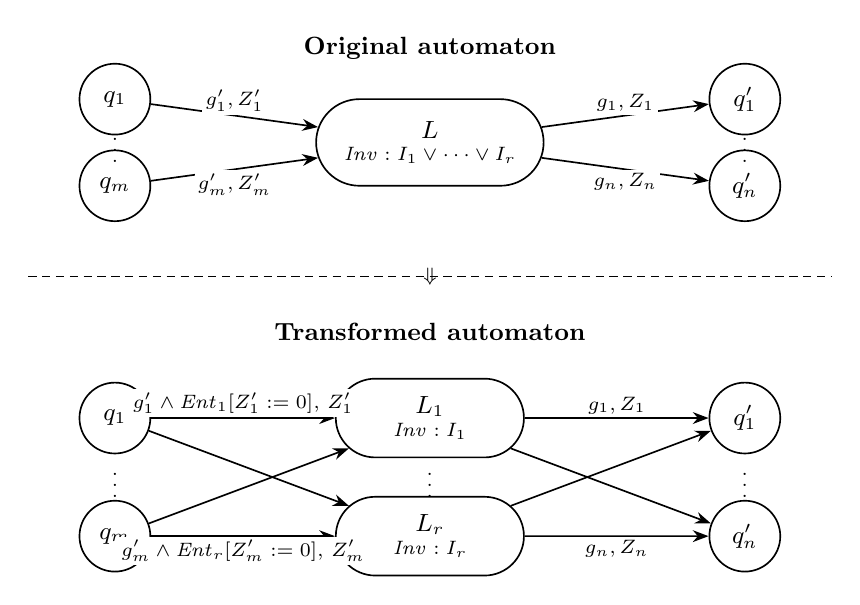
\begin{tikzpicture}[x=1cm,y=1cm]
  % Original automaton
  \node[font=\small\bfseries] at (0,3.45) {Original automaton};
\node[
  fmstatewide,minimum width=31mm,minimum height=11mm,
  align=center
] (L) at (0,2.25)
  {$L$\\[-1mm]{\scriptsize $\mathit{Inv}: I_1\lor\cdots\lor I_r$}};

  \node[fmstate] (q1) at (-4.0,2.8) {$q_1$};
  \node[fmstate] (qm) at (-4.0,1.7) {$q_m$};
  \node[fmnote] at (-4.0,2.25) {$\vdots$};
  \draw[fmedge] (q1) -- node[fmlabel,above] {$g'_1,Z'_1$} (L);
  \draw[fmedge] (qm) -- node[fmlabel,below] {$g'_m,Z'_m$} (L);

  \node[fmstate] (qp1) at (4.0,2.8) {$q'_1$};
  \node[fmstate] (qpn) at (4.0,1.7) {$q'_n$};
  \node[fmnote] at (4.0,2.25) {$\vdots$};
  \draw[fmedge] (L) -- node[fmlabel,above] {$g_1,Z_1$} (qp1);
  \draw[fmedge] (L) -- node[fmlabel,below] {$g_n,Z_n$} (qpn);

  \draw[fmguide] (-5.1,0.55) -- (5.1,0.55);
  \node[fmnote] at (0,0.55) {$\Downarrow$};

  % Transformed automaton
  \node[font=\small\bfseries] at (0,-0.15) {Transformed automaton};
  \node[fmstatewide,minimum width=26mm,minimum height=10mm,
  align=center] (L1) at (0,-1.25)
    {$L_1$\\[-1mm]\scriptsize $\mathit{Inv}: I_1$};

  \node[fmstatewide,minimum width=26mm,minimum height=10mm,
  align=center] (Lp) at (0,-2.75)
    {$L_r$\\[-1mm]\scriptsize $\mathit{Inv}: I_r$};
  \node[fmnote] at (0,-2.0) {$\vdots$};

  \node[fmstate] (r1) at (-4.0,-1.25) {$q_1$};
  \node[fmstate] (rm) at (-4.0,-2.75) {$q_m$};
  \node[fmnote] at (-4.0,-2.0) {$\vdots$};

  \draw[fmedge] (r1) -- node[fmlabel,above,sloped] {$g'_1\land \mathit{Ent}_1[Z'_1:=0],\,Z'_1$} (L1);
  \draw[fmedge] (r1) -- (Lp);
  \draw[fmedge] (rm) -- (L1);
  \draw[fmedge] (rm) -- node[fmlabel,below,sloped] {$g'_m\land \mathit{Ent}_r[Z'_m:=0],\,Z'_m$} (Lp);

  \node[fmstate] (s1) at (4.0,-1.25) {$q'_1$};
  \node[fmstate] (sn) at (4.0,-2.75) {$q'_n$};
  \node[fmnote] at (4.0,-2.0) {$\vdots$};

  \draw[fmedge] (L1) -- node[fmlabel,above] {$g_1,Z_1$} (s1);
  \draw[fmedge] (L1) -- (sn);
  \draw[fmedge] (Lp) -- (s1);
  \draw[fmedge] (Lp) -- node[fmlabel,below] {$g_n,Z_n$} (sn);
\end{tikzpicture}
}
\caption{Elimination of a disjunctive invariant. Each copy has a conjunctive invariant, and the entry guard selects a copy that admits a maximal delay from the incoming valuation. The entry condition can contain clock-difference constraints.}
\label{fig:disj-general}
\end{figure*}

The export continues by splitting disjunctive guards into conjunctive transitions, normalizing, pruning unreachable copies, and merging the initial location when an equivalent copy exists. A final symbolic pass groups transitions with the same source, target, and resets and stores their labels as Boolean conditions for drawings.

\begin{theorem}[Export preservation]
\label{thm:export}
For every automaton accepted by the verified export interface, the complete export preserves its timed-word language. The resulting explicit automaton has conjunctive transition guards and conjunctive location invariants. Its symbolic representation also preserves acceptance.
\end{theorem}
\begin{proof}
Export composes verified transition merging, invariant splitting, guard splitting, normalization, pruning, initial-location merging, and symbolic grouping. Each component has a language-preservation theorem, including \texttt{split\_accepts} for invariant elimination and \texttt{export\_accepts} for the complete construction. Output shape is established by \texttt{export\_guards\_conjunctive} and \texttt{export\_invariants\_conjunctive}.
\end{proof}
For reuse with another producer or checker, the theorem's output contract is
summarized in Table~\ref{tab:export-contract}.
\begin{table*}[t]
\centering
\caption{Contract of the verified optimization and export pipeline. The
explicit and symbolic outputs preserve the timed-word language of the TBA
provided to the Coq interface.}
\label{tab:export-contract}
\small
\begin{tabular}{@{}p{0.22\textwidth}p{0.70\textwidth}@{}}
\toprule
Aspect & Guaranteed result\\
\midrule
Timed-word language & Preserved by every optimization round and by complete export under the development's existential initial-clock semantics.\\
Explicit guards & Conjunctions of event literals and clock comparisons; export may introduce clock-difference comparisons in entry conditions.\\
Location invariants & Conjunctions of non-strict clock upper bounds.\\
Symbolic output & Groups transitions with the same source, target, and reset set under Boolean labels; the symbolic automaton also preserves acceptance.\\
Input adapter & A third-party parser or conversion into the Coq TBA representation requires a separate correspondence proof to join the verified boundary.\\
\bottomrule
\end{tabular}
\end{table*}
The complete construction and proof of the invariant split, including its entry-condition formula, appear in Section~\ref{subsec:disjunctive-invariants}. The theorem is generic in the automaton: it requires no MTL provenance, determinism, or particular Spot option.

\subsection{Generated automata with disjunctive invariants}
The following two tracked inputs show how the export handles disjunctive
invariants in automata produced by the integrated tool. They illustrate the
verified post-processing and export layer; the upstream translation is not
part of the generic preservation claims in this paper.

\subsubsection{Nested upper-bounded Until}
For
\[
  \Diamond_{\le5}(p\,\mathsf U_{\le2}\,q),
\]
the optimized automaton has a disjunctive invariant at location~4,
$x_{u1}\le2\lor x_{u0}\le5$. Every edge entering that location resets
$x_{u1}$. If the entry value of $x_{u0}$ is $v$, the two invariant clauses
permit delays of $2$ and $5-v$. The export splits location~4 into a copy with
invariant $x_{u1}\le2$ and a copy with invariant $x_{u0}\le5$. Their entry
conditions are respectively $x_{u0}\ge3$ and $x_{u0}\le3$: each selects a
copy that admits a maximal delay. Both are enabled at the tie $x_{u0}=3$.
Incoming transitions, including the self-loop, are replicated to both
copies, and outgoing transitions are replicated from each.

Figure~\ref{fig:ex1-invariants} shows the generated automaton before and after
the split. For readability, the drawing omits guards implied by source
invariants and edges subsumed by another edge with the same target, event,
and resets; the exported automaton retains them. The output has 23 explicit
transitions with \texttt{-init} (25 without it). This example uses Spot
options \texttt{-B -D}; dead resets have already been removed.

\begin{figure*}[!tp]
\centering
\subfloat[Before invariant elimination.\label{fig:ex1-with-disj}]{
  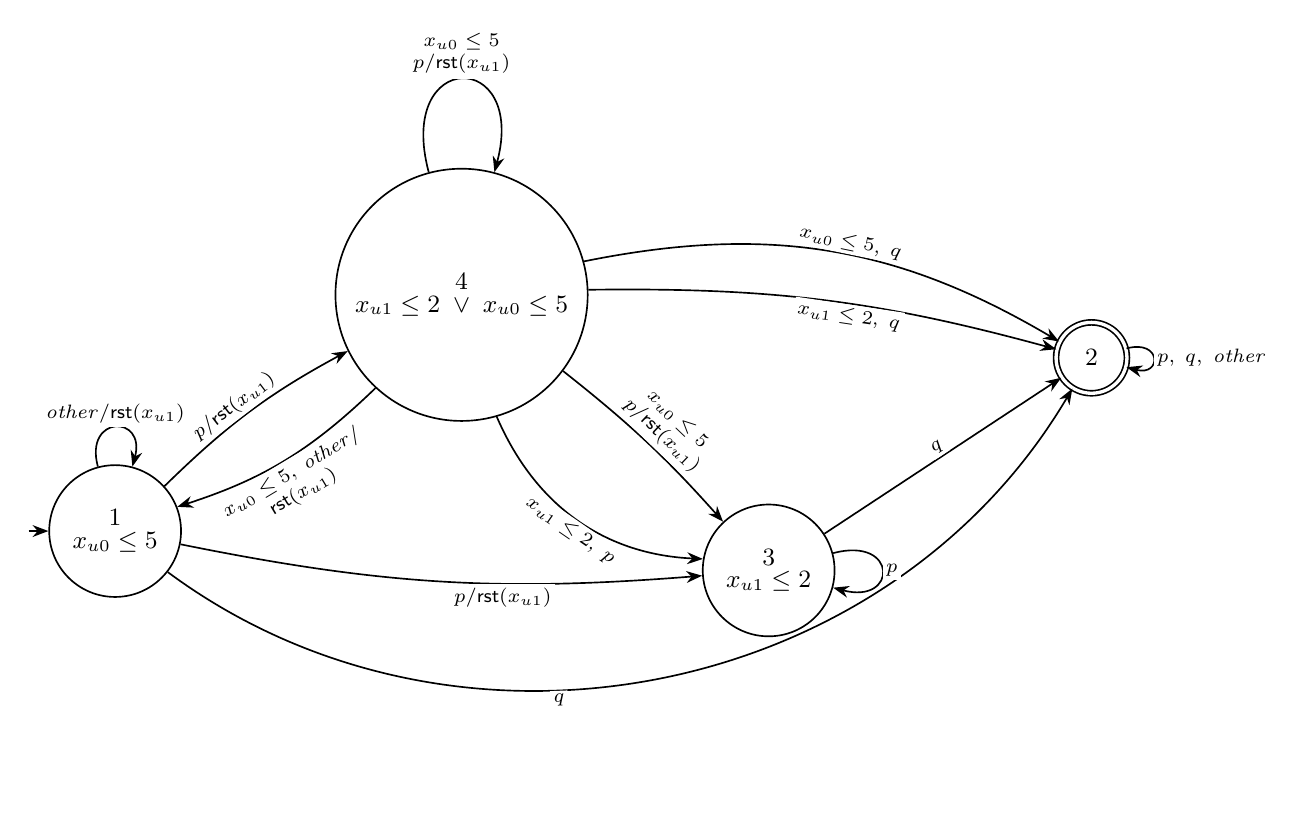
\begin{tikzpicture}[x=1cm,y=1cm]
  \node[fmstate,minimum size=13mm] (s1) at (0,0) {$\begin{array}{c}1\\[-1mm]x_{u0}\le5\end{array}$};
  \node[fmstate,minimum size=18mm] (s4) at (4.4,3.0) {$\begin{array}{c}4\\[-1mm]x_{u1}\le2\;\lor\;x_{u0}\le5\end{array}$};
  \node[fmstate,minimum size=14mm] (s3) at (8.3,-0.5) {$\begin{array}{c}3\\[-1mm]x_{u1}\le2\end{array}$};
  \node[fmaccept] (s2) at (12.4,2.2) {$2$};
  \draw[fmedge] (-1.1,0) -- (s1);
  \draw[fmedge] (s1) edge[loop above,looseness=4] node[fmlabel] {$\mathit{other}/\mathsf{rst}(x_{u1})$} (s1);
  \draw[fmedge] (s1) to[bend left=8] node[fmlabel,pos=.45,above,sloped] {$p/\mathsf{rst}(x_{u1})$} (s4);
  \draw[fmedge] (s4) to[bend left=13] node[fmlabel,pos=.50,below,sloped] {$\begin{array}{c}x_{u0}\le5,\;\mathit{other}/\\\mathsf{rst}(x_{u1})\end{array}$} (s1);
  \draw[fmedge] (s1) to[bend right=8] node[fmlabel,pos=.63,below] {$p/\mathsf{rst}(x_{u1})$} (s3);
  \draw[fmedge] (s1) to[bend right=48] node[fmlabel,pos=.4,below,sloped] {$q$} (s2);
  \draw[fmedge] (s4) edge[loop above,looseness=5] node[fmlabel] {$\begin{array}{c}x_{u0}\le5\\p/\mathsf{rst}(x_{u1})\end{array}$} (s4);
  \draw[fmedge] (s4) to[bend left=21] node[fmlabel,pos=.54,above,sloped] {$x_{u0}\le5,\;q$} (s2);
  \draw[fmedge] (s4) to[bend left=8] node[fmlabel,pos=.56,below,sloped] {$x_{u1}\le2,\;q$} (s2);
  \draw[fmedge] (s4) to[bend left=5] node[fmlabel,pos=.53,above,sloped] {$\begin{array}{c}x_{u0}\le5\\p/\mathsf{rst}(x_{u1})\end{array}$} (s3);
  \draw[fmedge] (s4) to[bend right=32] node[fmlabel,pos=.5,below,sloped] {$x_{u1}\le2,\;p$} (s3);
  \draw[fmedge] (s3) edge[loop right,looseness=5] node[fmlabel,right] {$p$} (s3);
  \draw[fmedge] (s3) -- node[fmlabel,above,sloped] {$q$} (s2);
  \draw[fmedge] (s2) edge[loop right,looseness=5] node[fmlabel,right] {$p,\;q,\;\mathit{other}$} (s2);
\end{tikzpicture}
}

\medskip

\subfloat[After invariant elimination.\label{fig:ex1-no-disj}]{
  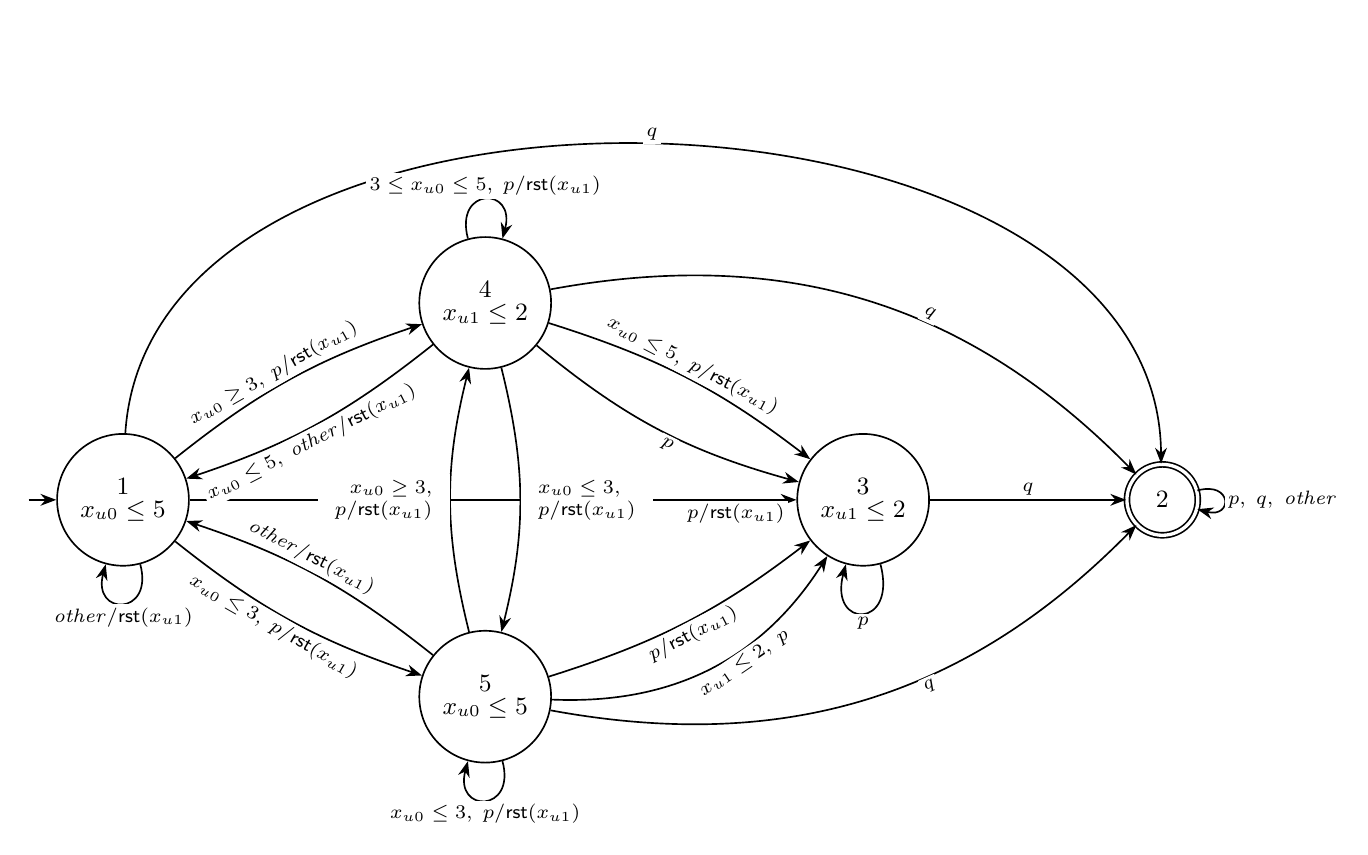
\begin{tikzpicture}[x=1cm,y=1cm]
  % Location 4 of the original automaton is split into 4 (Inv x_u1<=2) and 5 (Inv x_u0<=5).
  % Every entry into the split location resets x_u1, so copy 4 allows a delay of 2 and
  % copy 5 a delay of 5 - x_u0; the entry guards select the copy with the longer delay.
  \node[fmstate,minimum size=13mm] (s1) at (0,0) {$\begin{array}{c}1\\[-1mm]x_{u0}\le5\end{array}$};
  \node[fmstate,minimum size=14mm] (s4) at (4.6,2.5) {$\begin{array}{c}4\\[-1mm]x_{u1}\le2\end{array}$};
  \node[fmstate,minimum size=14mm] (s5) at (4.6,-2.5) {$\begin{array}{c}5\\[-1mm]x_{u0}\le5\end{array}$};
  \node[fmstate,minimum size=14mm] (s3) at (9.4,0) {$\begin{array}{c}3\\[-1mm]x_{u1}\le2\end{array}$};
  \node[fmaccept] (s2) at (13.2,0) {$2$};
  \draw[fmedge] (-1.2,0) -- (s1);
  % location 1
  \draw[fmedge] (s1) edge[loop below,looseness=4] node[fmlabel,below] {$\mathit{other}/\mathsf{rst}(x_{u1})$} (s1);
  \draw[fmedge] (s1) to[bend left=10] node[fmlabel,pos=.45,above,sloped] {$x_{u0}\ge3,\;p/\mathsf{rst}(x_{u1})$} (s4);
  \draw[fmedge] (s1) to[bend right=10] node[fmlabel,pos=.45,below,sloped] {$x_{u0}\le3,\;p/\mathsf{rst}(x_{u1})$} (s5);
  \draw[fmedge] (s1) -- node[fmlabel,pos=.9,below] {$p/\mathsf{rst}(x_{u1})$} (s3);
  \draw[fmedge] (s1) to[bend left=88] node[fmlabel,above] {$q$} (s2);
  % location 4 (Inv x_u1 <= 2)
  \draw[fmedge] (s4) to[bend left=10] node[fmlabel,pos=.55,below,sloped] {$x_{u0}\le5,\;\mathit{other}/\mathsf{rst}(x_{u1})$} (s1);
  \draw[fmedge] (s4) edge[loop above,looseness=4] node[fmlabel,above] {$3\le x_{u0}\le5,\;p/\mathsf{rst}(x_{u1})$} (s4);
  \draw[fmedge] (s4) to[bend left=14] node[fmlabel,right] {$\begin{array}{l}x_{u0}\le3,\\p/\mathsf{rst}(x_{u1})\end{array}$} (s5);
  \draw[fmedge] (s4) to[bend left=10] node[fmlabel,pos=.5,above,sloped] {$x_{u0}\le5,\;p/\mathsf{rst}(x_{u1})$} (s3);
  \draw[fmedge] (s4) to[bend right=12] node[fmlabel,pos=.55,below,sloped] {$p$} (s3);
  \draw[fmedge] (s4) to[bend left=28] node[fmlabel,pos=.6,above,sloped] {$q$} (s2);
  % location 5 (Inv x_u0 <= 5)
  \draw[fmedge] (s5) to[bend right=10] node[fmlabel,pos=.55,above,sloped] {$\mathit{other}/\mathsf{rst}(x_{u1})$} (s1);
  \draw[fmedge] (s5) edge[loop below,looseness=4] node[fmlabel,below] {$x_{u0}\le3,\;p/\mathsf{rst}(x_{u1})$} (s5);
  \draw[fmedge] (s5) to[bend left=14] node[fmlabel,left] {$\begin{array}{r}x_{u0}\ge3,\\p/\mathsf{rst}(x_{u1})\end{array}$} (s4);
  \draw[fmedge] (s5) to[bend right=10] node[fmlabel,pos=.5,below,sloped] {$p/\mathsf{rst}(x_{u1})$} (s3);
  \draw[fmedge] (s5) to[bend right=30] node[fmlabel,pos=.6,below,sloped] {$x_{u1}\le2,\;p$} (s3);
  \draw[fmedge] (s5) to[bend right=28] node[fmlabel,pos=.6,below,sloped] {$q$} (s2);
  % locations 3 and 2
  \draw[fmedge] (s3) edge[loop below,looseness=5] node[fmlabel,below] {$p$} (s3);
  \draw[fmedge] (s3) -- node[fmlabel,above] {$q$} (s2);
  \draw[fmedge] (s2) edge[loop right,looseness=5] node[fmlabel,right] {$p,\;q,\;\mathit{other}$} (s2);
\end{tikzpicture}
}
\caption{Generated automaton for $\Diamond_{\le5}(p\,\mathsf U_{\le2}\,q)$.
Location invariants appear inside the nodes; edge labels are ``guard, event /
resets.'' A comma-separated event list denotes separate transitions, and
$\mathit{other}$ denotes any event other than $p$ and $q$. The double circle
marks the accepting location. Both diagrams are after the initial
\texttt{\_init\_} transition at time zero. Location~5 is created by the
split. Guards implied by source invariants and subsumed edges are omitted from
the drawing.}
\label{fig:ex1-invariants}
\end{figure*}
At the timed-word level, the accepted behavior has a direct witness: either
$q$ occurs at a position $k$ with $t_k\le5$, or a sequence satisfying $p$
starts at some $j$ with $t_j\le5$ and reaches $q$ at $k$ with
$t_k-t_j\le2$. The split preserves these same choices at location~4 while
making each location invariant conjunctive.

\subsubsection{Timed Release obligation inside Until}
The second input is
\[
  \Diamond_{\le5}\bigl((\Box_{\le3}(p\lor q))\,\mathsf U_{\le2}\,q\bigr).
\]
Its optimized automaton has seven locations before export and contains a
disjunctive invariant (Fig.~\ref{fig:ex2-disj}). The three distinct primitive
timed subformulas use clocks $x_{u0}$, $x_{u1}$, and $x_{r2}$. Two syntactic
occurrences of the bounded Release share $x_{r2}$ because the clock key is
the primitive formula.

When a $q$ transition enters accepting location~5, the automaton permits only
$p$ or $q$ until $x_{r2}>3$, after which location~2 accepts every event. The
bounded Release obligation can therefore remain pending after the Until
witness. Two $q$ transitions testing $x_{r2}>3$ are unsatisfiable: at
location~4, entry resets both relevant clocks; at location~3, entry resets
$x_{r2}$ and preserves $x_{u1}$ with $x_{r2}\le x_{u1}\le2$. The verified
passes compare clock bounds with constants and do not track this clock-order
relation, so the transitions remain in the optimized drawing. They cannot be
taken. Export produces seven locations and 29 transitions.

\begin{figure*}[!t]
\centering
\resizebox{\textwidth}{!}{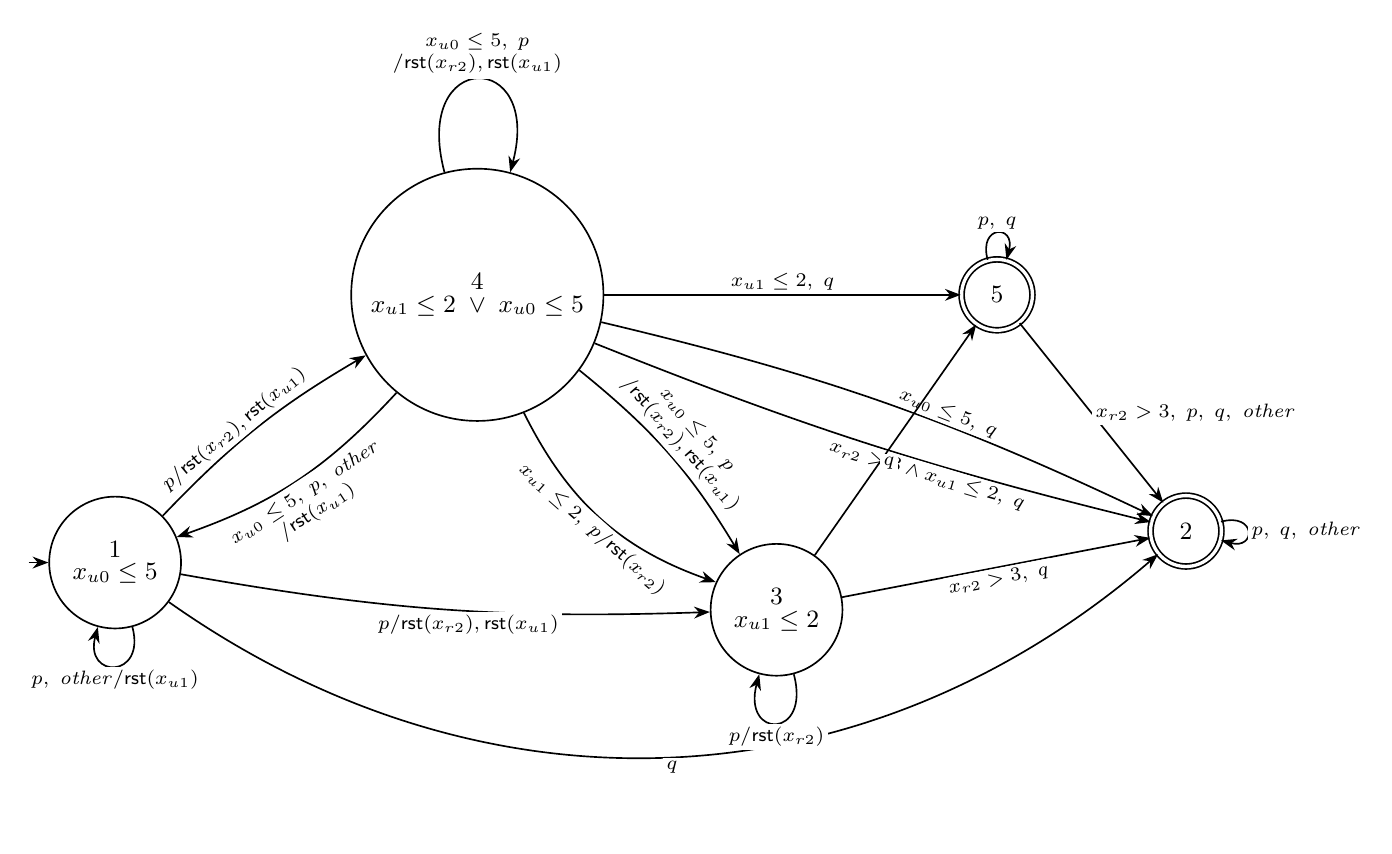
\begin{tikzpicture}[x=1cm,y=1cm]
  % Output of mtl2tba -init after optimization, before the export
  % (clocks printed x0, x1, x2 by the tool are x_u0, x_r2, x_u1).
  \node[fmstate,minimum size=13mm] (s1) at (0,0) {$\begin{array}{c}1\\[-1mm]x_{u0}\le5\end{array}$};
  \node[fmstate,minimum size=19mm] (s4) at (4.6,3.4) {$\begin{array}{c}4\\[-1mm]x_{u1}\le2\;\lor\;x_{u0}\le5\end{array}$};
  \node[fmstate,minimum size=14mm] (s3) at (8.4,-0.6) {$\begin{array}{c}3\\[-1mm]x_{u1}\le2\end{array}$};
  \node[fmaccept] (s5) at (11.2,3.4) {$5$};
  \node[fmaccept] (s2) at (13.6,0.4) {$2$};
  \draw[fmedge] (-1.1,0) -- (s1);
  % location 1
  \draw[fmedge] (s1) edge[loop below,looseness=4] node[fmlabel,below] {$p,\;\mathit{other}/\mathsf{rst}(x_{u1})$} (s1);
  \draw[fmedge] (s1) to[bend left=8] node[fmlabel,pos=.42,above,sloped] {$p/\mathsf{rst}(x_{r2}),\mathsf{rst}(x_{u1})$} (s4);
  \draw[fmedge] (s1) to[bend right=6] node[fmlabel,pos=.55,below] {$p/\mathsf{rst}(x_{r2}),\mathsf{rst}(x_{u1})$} (s3);
  \draw[fmedge] (s1) to[bend right=38] node[fmlabel,pos=.5,below] {$q$} (s2);
  % location 4
  \draw[fmedge] (s4) to[bend left=14] node[fmlabel,pos=.5,below,sloped] {$\begin{array}{c}x_{u0}\le5,\;p,\;\mathit{other}\\/\mathsf{rst}(x_{u1})\end{array}$} (s1);
  \draw[fmedge] (s4) edge[loop above,looseness=5] node[fmlabel] {$\begin{array}{c}x_{u0}\le5,\;p\\/\mathsf{rst}(x_{r2}),\mathsf{rst}(x_{u1})\end{array}$} (s4);
  \draw[fmedge] (s4) to[bend left=10] node[fmlabel,pos=.5,above,sloped] {$\begin{array}{c}x_{u0}\le5,\;p\\/\mathsf{rst}(x_{r2}),\mathsf{rst}(x_{u1})\end{array}$} (s3);
  \draw[fmedge] (s4) to[bend right=22] node[fmlabel,pos=.5,below,sloped] {$x_{u1}\le2,\;p/\mathsf{rst}(x_{r2})$} (s3);
  \draw[fmedge] (s4) -- node[fmlabel,above] {$x_{u1}\le2,\;q$} (s5);
  \draw[fmedge] (s4) to[bend left=6] node[fmlabel,pos=.62,above,sloped] {$x_{u0}\le5,\;q$} (s2);
  \draw[fmedge] (s4) to[bend right=4] node[fmlabel,pos=.62,below,sloped] {$x_{r2}>3\land x_{u1}\le2,\;q$} (s2);
  % location 3
  \draw[fmedge] (s3) edge[loop below,looseness=5] node[fmlabel,below] {$p/\mathsf{rst}(x_{r2})$} (s3);
  \draw[fmedge] (s3) -- node[fmlabel,right,pos=.4] {$q$} (s5);
  \draw[fmedge] (s3) -- node[fmlabel,below,sloped] {$x_{r2}>3,\;q$} (s2);
  % location 5
  \draw[fmedge] (s5) edge[loop above,looseness=5] node[fmlabel] {$p,\;q$} (s5);
  \draw[fmedge] (s5) -- node[fmlabel,right] {$x_{r2}>3,\;p,\;q,\;\mathit{other}$} (s2);
  \draw[fmedge] (s2) edge[loop right,looseness=5] node[fmlabel,right] {$p,\;q,\;\mathit{other}$} (s2);
\end{tikzpicture}
}
\caption{Optimized automaton for
$\Diamond_{\le5}((\Box_{\le3}(p\lor q))\,\mathsf U_{\le2}\,q)$ before
disjunctive-invariant elimination. Clocks $x_{u0}$, $x_{u1}$, and $x_{r2}$
belong to the three distinct primitive timed subformulas. The diagram is
after the initial \texttt{\_init\_} transition; guards implied by source
invariants are omitted. A comma-separated event list denotes separate
transitions. The $q$-edges from locations~4 and~3 with $x_{r2}>3$ are
unsatisfiable for the reasons given in the text.}
\label{fig:ex2-disj}
\end{figure*}

\subsubsection{Optimization and export of the F11 automaton}
The F11 automaton for
$ (\Diamond_{\le5}p)\land(\Box_{<2}\neg p) $ illustrates the interaction
between the generic passes. Spot returns five states and eleven transitions.
After one optimization round, contradictory action cubes have been removed,
making location~2 unreachable; dead resets are removed, and clocks $x$ and
$y$ are merged because every transition resets them synchronously. The
second round removes the now-dead resets of $y$. The final UPPAAL-oriented
automaton has four locations, seven transitions, one clock, and two location
invariants. Figure~\ref{fig:running-pipeline} shows the state after the first
round and the exported form. This example concerns the optimizer and export;
its temporal translation is handled separately.

\begin{figure*}[!t]
\centering
\resizebox{\textwidth}{!}{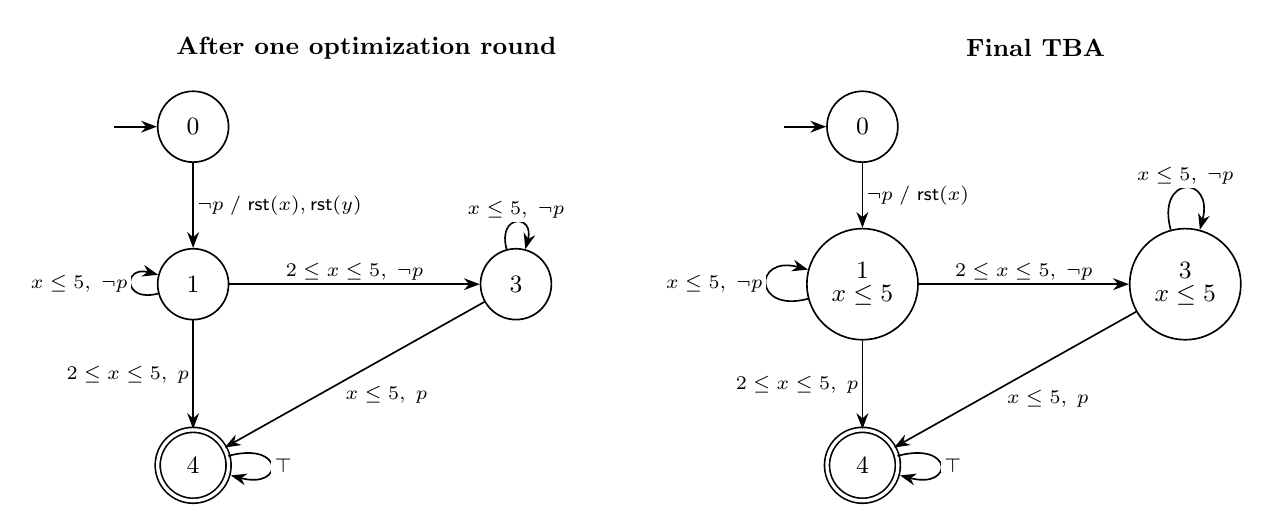
\begin{tikzpicture}[x=1cm,y=1cm,lab/.style={fmlabel}]
\begin{scope}[xshift=0cm]
  \node[fmnote,font=\small\bfseries] at (2.2,5.3) {After one optimization round};
  \node[fmstate] (l0) at (0.0,4.3) {$0$};
  \node[fmstate] (l1) at (0.0,2.3) {$1$};
  \node[fmstate] (l3) at (4.1,2.3) {$3$};
  \node[fmaccept] (l4) at (0.0,0.0) {$4$};
  \draw[fmedge] (-1.0,4.3) -- (l0);
  \draw[fmedge] (l0) -- node[lab,right] {$\neg p\;/\;\mathsf{rst}(x),\mathsf{rst}(y)$} (l1);
  \draw[fmedge] (l1) edge[loop left,looseness=5] node[lab,left] {$x\le5,\;\neg p$} (l1);
  \draw[fmedge] (l1) -- node[lab,above] {$2\le x\le5,\;\neg p$} (l3);
  \draw[fmedge] (l1) -- node[lab,left] {$2\le x\le5,\;p$} (l4);
  \draw[fmedge] (l3) edge[loop above,looseness=5] node[lab,above] {$x\le5,\;\neg p$} (l3);
  \draw[fmedge] (l3) -- node[lab,pos=.55,below right] {$x\le5,\;p$} (l4);
  \draw[fmedge] (l4) edge[loop right] node[lab,right] {$\top$} (l4);
\end{scope}

\begin{scope}[xshift=8.5cm]
  \node[fmnote,font=\small\bfseries] at (2.2,5.3) {Final TBA};
  \node[fmstate] (r0) at (0.0,4.3) {$0$};
  \node[fmstate,minimum size=11mm] (r1) at (0.0,2.3) {$\begin{array}{c}1\\[-1mm]x\le5\end{array}$};
  \node[fmstate,minimum size=11mm] (r3) at (4.1,2.3) {$\begin{array}{c}3\\[-1mm]x\le5\end{array}$};
  \node[fmaccept] (r4) at (0.0,0.0) {$4$};
  \draw[fmedge] (-1.0,4.3) -- (r0);
  \draw[fmedge] (r0) -- node[lab,right] {$\neg p\;/\;\mathsf{rst}(x)$} (r1);
  \draw[fmedge] (r1) edge[loop left,looseness=5] node[lab,left] {$x\le5,\;\neg p$} (r1);
  \draw[fmedge] (r1) -- node[lab,above] {$2\le x\le5,\;\neg p$} (r3);
  \draw[fmedge] (r1) -- node[lab,left] {$2\le x\le5,\;p$} (r4);
  \draw[fmedge] (r3) edge[loop above,looseness=5] node[lab,above] {$x\le5,\;\neg p$} (r3);
  \draw[fmedge] (r3) -- node[lab,pos=.55,below right] {$x\le5,\;p$} (r4);
  \draw[fmedge] (r4) edge[loop right] node[lab,right] {$\top$} (r4);
\end{scope}
\end{tikzpicture}
}
\caption{F11 after one optimization round and after UPPAAL-oriented export.
The first panel shows the removed unreachable location and the two
synchronously reset clocks; the final panel shows the merged clock and
synthesized invariants. Edges use the form ``guard, action / resets,'' and the
double circle marks the accepting location.}
\label{fig:running-pipeline}
\end{figure*}


\section{Tool Architecture and Use in UPPAAL}
\label{sec:toolchain}
\subsection{Implementation and proof boundary}
The OCaml module \texttt{optim.ml} is extracted from Coq. It implements the invariant and optimization functions, export passes, initialization check used by the upstream MTL workflow, and symbolic grouping. The surrounding \texttt{mtl2tba} executable contains a hand-written parser, calls Spot when building its upstream automaton, reads the returned LBTT automaton, drives the optimization loop, and prints UPPAAL XML and Graphviz DOT. In generic use, the verified functions operate on their Coq TBA type; a parser or converter for a third-party TBA format is an additional trusted interface unless verified separately.

Pass theorems are independent of the source of their TBA. End-to-end correctness for an MTL formula additionally composes with the upstream translation and its linear temporal logic (LTL)-to-B\"uchi contract. The Spot call, parser, LBTT reader, driver, and XML/DOT printers are outside the Coq pass proofs. The floating-point realization of extracted real-number operations is also trusted; the tool restricts bounds to integers in $[0,2^{30}]$, for which inspected arithmetic is exact in the target representation. The repository records Rocq 9.0.1, OCaml 5.4.0, Spot 2.16, and UPPAAL 5.0.0 for the build and case-study artifacts.

The project-wide axiom \texttt{LTL\_TO\_BUCHI\_CORRECT} states the assumed
correctness of the upstream LTL-to-B\"uchi backend. It is used by the
end-to-end theorem variants that do not take the backend contract as an
explicit argument. The generic \texttt{optimize\_accepts} and
\texttt{export\_accepts} theorems instead quantify over an arbitrary TBA and
do not use that axiom; their proof boundary is the timed-word semantics of
the input automaton.

In the integrated executable, Spot is called with state-based B\"uchi output,
the small-automaton option, and LBTT transition labels. Clock predicates,
event markers, and action literals are supplied as separate propositions, as
required by the upstream translation contract. The hand-written reader
retains positive and negative literals and expands each transition label into
its cubes. The extracted functions then perform relaxation and reset
completion, run the optimizer until the automaton stops changing or 50 rounds
have elapsed, and apply the UPPAAL-oriented export. The proof is independent
of this particular command and front end; the sequence describes how the
generic verified layer is used in the available tool.

The generic theorems use existential initial clock values. UPPAAL starts clocks at zero. The verified \texttt{init\_free} check and its zero-initialization theorem are part of the MTL-generated workflow; they do not provide an initialization theorem for arbitrary third-party TBAs. Users should check the initialization contract of any external automaton.

\subsection{Input contract for a generic TBA}
\label{sec:generic-input}
The generic interface starts from a finite TBA value
$(L,\ell_0,X,E,\mathit{Acc})$ in the Coq representation. Its transitions carry
event conditions, finite conjunctions of unary clock comparisons, and reset
sets; the starting value has no location-invariant annotation. The invariant
synthesis pass derives that annotation from outgoing guards. The theorem
does not require a complete or deterministic transition relation, a particular
number of clocks, or a connection to a temporal-logic translator. A third-party
producer can therefore use the proved functions after converting its automaton
to this representation.

The conversion is a semantic boundary: it must retain the alphabet and the
meaning of each event condition, preserve which clocks are tested and reset,
and map accepting locations without changing their marking. The paper's
repository provides the Coq type and extracted optimizer, but not a verified
reader for arbitrary third-party formats. Any such reader belongs to the
trusted interface until its correspondence with the Coq value is proved. The
same applies to interpreting the result in a target checker: export proves
language preservation for the Coq representation, while a separate bridge is
needed to identify the checker's parsed model with that value. This boundary
allows the central optimization theorem to remain generic while making the
work needed to reuse it explicit.

\subsection{Initialization interface}
For the integrated MTL workflow, the verified \texttt{init\_free} check
establishes that the output language is unchanged when clocks start at zero.
It succeeds on each completed default benchmark instance; R7 and R8 exceed
the 300-second construction limit before producing an output. If the check
fails, the driver can use \texttt{-init}, which inserts a single
\texttt{\_init\_} event at time zero and rewrites the formula so that ordinary
top-level timing bounds use that temporal origin. The system model must emit
this event exactly once before its other events. This hand-written
transformation is argued in the artifact but is not part of the generic
optimization or export theorem. On the tracked benchmark, \texttt{-init}
keeps the clock count unchanged, adds at most one location, and changes the
transition count by between twelve fewer and one more than the default
output. These are measured properties of the integrated workflow.

\subsection{Using exported automata in UPPAAL}
The language-preservation theorem concerns infinite timed words with one
event at each position, strictly increasing timestamps, divergent time, and
the development's clock initialization semantics. A UPPAAL composition must
preserve the assumptions needed to interpret its traces in that model:
\begin{enumerate}[label=(C\arabic*),leftmargin=*]
  \item \emph{Events and time.} The system must synchronize each observable
        event with the property automaton, prevent zero-delay consecutive
        events (for example, reset a system clock $z$ on each emission and
        require $z>0$ on the next), and admit time-divergent infinite
        executions. Reachability alone does not rule out a Zeno continuation.
  \item \emph{Initial clocks.} The generic Coq preservation theorems
        existentially quantify over initial clock values. UPPAAL initializes
        clocks to zero. The tool's verified \texttt{init\_free} check supplies
        a zero-initialization result for the MTL-generated workflow when it
        succeeds; it is not a generic guarantee for a third-party TBA.
  \item \emph{Acceptance.} UPPAAL's ordinary reachability interface does not
        check B\"uchi acceptance. For safety, use a violation automaton with
        an accepting sink that is reached when a violation occurs and has a
        loop on every event. Liveness requires a B\"uchi emptiness checker
        that restricts attention to time-divergent runs; the artifact uses
        TChecker for this task.
  \item \emph{Time constraints in products.} Location invariants are part of
        the automaton semantics and can block time in a product, thereby
        removing system behaviors. An exported property automaton is not a
        passive observer unless its effect on the product is separately
        justified. Check deadlock or timelock conditions on the system as
        appropriate.
  \item \emph{Numbers.} The integrated tool accepts integer bounds in
        $[0,2^{30}]$. The Coq theorems are over real-valued clocks; the
        extracted implementation's arithmetic and the UPPAAL printer are
        covered only on the tool's restricted numeric domain.
\end{enumerate}

The generated XML has a \texttt{Property} template for the automaton and an
\texttt{Env} template that can emit events for standalone language
exploration. In a system check, the system replaces \texttt{Env} and
synchronizes its observable events with \texttt{Property}; the event
\texttt{other} denotes any event outside the finite set named in the formula.
Accepting locations are named \texttt{A}$n$ in the output, but those names do
not make UPPAAL check B\"uchi acceptance. For a safety requirement, the
reachability query must use an automaton for its violations with a sink entered
once the violation has occurred. For a liveness requirement, reachability of
such a sink is not the right check and an emptiness procedure for
time-divergent B\"uchi runs is needed.

For a safety property $\varphi$, let $\mathcal A_{\neg\varphi}$ be a
violation automaton whose accepting sink has no invariant and loops on every
event. Compose it with a system $S$ that synchronizes the same event alphabet
and can extend every queried prefix to a time-divergent execution. Under
(C1)--(C3) and the appropriate initialization condition in (C2), the query
\texttt{E<> P.A} detects a system behavior violating $\varphi$ when the
automaton recognizes exactly those violations. This query-level equivalence
is an argument about the chosen system and automaton; it is not proved by the
generic Coq optimization or export theorem. The case-study models below
report the model checks and diagnostic traces for the four packaged systems.

\subsection{Availability}
This project contains proof sources, extracted implementation, benchmark tables and raw data, reproduction scripts, and UPPAAL case-study models, together with the LaTeX source and build instructions. The authors' earlier mtl2tba v1.10 tool and proof artifacts document the integrated MTL-to-TBA workflow~\cite{mtl2b_tool,mtl2b_proof}; this article focuses on its generic TBA-level optimization and export contracts. The invariant, optimization, and export formalization files contain the generic pass results; their theorem names are listed in Table~\ref{tab:post-passes}. The project repository is at \url{https://github.com/efares1/verified-tba-optimization-uppaal}.

\subsection{Build and artifact layout}
The verified functions are defined under \texttt{proof/} and extracted into
\texttt{tool/src/optim.ml}. The project Makefile compiles the Rocq
development and extracts the executable functions. Hand-written components
include the parser, Spot invocation, LBTT reader, iteration driver, and
XML/DOT printers; the script that removes unreachable extracted definitions
and the Rocq/OCaml toolchains are also part of the implementation's trusted
base. The repository includes the machine record, raw benchmark runs, TSV
summaries, table generator, formulas, UPPAAL models and queries, and
reproduction instructions in \texttt{README.md}.

Table~\ref{tab:component-boundary} separates the verified transformations
from the interfaces that connect them to the surrounding tools.
\begin{table*}[t]
\centering
\caption{Runtime stages and their proof boundary. The generic theorems begin
with a TBA in the Coq representation; the Spot-based formula front end is one
client of the verified optimizer and exporter.}
\label{tab:component-boundary}
\footnotesize
\begin{tabular}{@{}p{0.22\textwidth}p{0.35\textwidth}p{0.35\textwidth}@{}}
\toprule
Stage & Implementation & Guarantee or boundary\\
\midrule
TBA input and adapter & Coq TBA value or a parser/converter supplied by the caller & Generic pass results start at this representation; an external adapter is outside the theorem unless separately verified.\\
Spot-based front end & Spot call and hand-written LBTT reader in \texttt{mtl2tba} & Used by the integrated formula workflow; outside the generic TBA theorem.\\
Optimization rounds & Extracted from \texttt{MTL\_to\_TBA\_Optimizations.v} & \texttt{optimize\_accepts}, for every TBA and every round count.\\
Iteration driver & Hand-written OCaml structural comparison; stops at equality or 50 rounds & The proof does not assume convergence or a particular stopping point.\\
UPPAAL export & Extracted from \texttt{MTL\_to\_TBA\_Export.v} & \texttt{export\_accepts} and conjunctive guard/invariant results.\\
Symbolic grouping & Extracted from \texttt{MTL\_to\_TBA\_Symbolic.v} & \texttt{symbolic\_ext\_accepts}.\\
XML, DOT, and PDF output & Hand-written printers and Graphviz & Outside the Coq language-preservation results.\\
Numeric realization & OCaml floating point with integer bounds in $[0,2^{30}]$ & Exactness follows from inspection of the extracted operations, not a mechanized theorem.\\
\bottomrule
\end{tabular}
\end{table*}

In the extracted code, structural equality decides formula and clock
identity, and Boolean checks implement conditions whose soundness is proved
in Coq. Real comparisons are realized by OCaml floating-point operations.
Input constants lie in $[0,2^{30}]$; the inspected operations produce only
such constants, their differences, or their negations. These values are
exactly representable by the 53-bit significand of a double, and the printed
constants fit UPPAAL's 32-bit integer domain. This arithmetic argument is
based on inspection of the extracted implementation rather than a theorem
about OCaml or the printer. Rational constants can be handled by a common time
scaling only when every scaled bound remains an integer in $[0,2^{30}]$; timing
constants in any surrounding system model must be scaled by the same factor.

\section{Evaluation}
\label{sec:evaluation}
\subsection{Questions and setup}
The evaluation addresses three questions: (1) what structural changes do optimization and export make on the current tool's benchmark automata; (2) how does the pipeline scale on conjunctions of bounded responses and nested bounded eventualities; and (3) do the output models support the included UPPAAL and timed-language checks? These are artifact and benchmark questions. The evaluation does not compare downstream checker runtime or memory before and after preprocessing; the measured benefit is verified normalization, output compatibility, and the structural changes reported below. The correctness theorems are universal in the input TBA, but measured inputs come from the current MTL-to-TBA workflow.

The tracked benchmark contains 31 configurations: requirement patterns F1--F14 and F3b; R$n$, which conjoins $n$ bounded responses for $1\le n\le8$; and N$n$, a nested bounded-eventuality family for $1\le n\le8$. The evaluation script attempts each configuration up to five times with a 300-second limit and stops after the first failed run. Successful configurations have five runs; R7 and R8 each have one timeout attempt. Reported stage and total times are medians of the successful runs. Full structural rows, run ranges, memory, and back-end comparisons appear in Tables~\ref{tab:evaluation} and~\ref{tab:scaling}; exact formulas are in Table~\ref{tab:formulas}. Runs used Ubuntu 26.04 under WSL 2 on an Intel Core i7-8650U at 1.9 GHz with 11.7 GB memory, Rocq 9.0.1, OCaml 5.4.0, and Spot 2.16. CASAAL, an MTL-to-timed-B\"uchi translator~\cite{casaal_tool}, ran natively on Windows on the same machine, so timing comparisons across operating systems are indicative only. UPPAAL case studies used version 5.0.0.

Table~\ref{tab:evaluation} gives the complete structural and timing results for all 31 configurations; exact input formulas are listed in Table~\ref{tab:formulas}.
\begin{table*}[t]
\centering
\caption{Evaluation of \texttt{mtl2tba} and comparison with CASAAL on the common semantic domain (one event per position).  $|X|$: number of distinct primitive (hatted) timed subformulas after unfolding of the ordinary operators and the default rewritings.  Spot: B\"uchi automaton returned by Spot (states/transitions, one transition per cube).  Opt.: after reset completion and the verified optimizations (locations/transitions/clocks).  Export: automaton for UPPAAL (locations, transitions, clocks, locations with an invariant, and occurrences of difference constraints in the guards).  Sym.: transitions of the symbolic automaton, with Boolean labels.  Time: wall-clock time, median of five runs of the whole chain including Spot, in seconds.  st, tr, loc, clk: states, transitions, locations, clocks.  CASAAL: states/transitions/clocks of the automaton of CASAAL for the formula conjoined with the mutual exclusion of its propositions; transitions carry Boolean formulas.  $\dagger$: not equivalent (CASAAL has no hatted operator); $\ddagger$: degenerate formula, equivalent to $\Box\neg p$ or $\Box\neg e$ with one event per position.  CASAAL time: wall-clock time, median of five runs, in seconds, including the start of the process.  TO: the chain exceeds the limit of 300~s (wall-clock, per run).  Lang.: comparison of the languages with those of CASAAL by TChecker (Section~\ref{main-sec:evaluation}, paragraph ``Comparison of languages with CASAAL''): exp, inclusion of the languages of CASAAL's automata into ours established on the exported automaton; cmp, established only on the automaton $\mathsf{compile}(f)$ before post-processing; ?, no conclusion within the limits; --, formulas not equivalent.  Equal sizes do not by themselves imply equal languages.  Formulas: Table~\ref{tab:formulas} of the supplementary material.}
\label{tab:evaluation}
\small
\setlength{\tabcolsep}{4.5pt}
\begin{tabular}{@{}lrrrrrrrrrrrrrrrc@{}}
\toprule
 & & \multicolumn{2}{c}{Spot} & \multicolumn{3}{c}{Opt.} & \multicolumn{5}{c}{Export} & & & \multicolumn{2}{c}{CASAAL} & \\
\cmidrule(lr){3-4}\cmidrule(lr){5-7}\cmidrule(lr){8-12}\cmidrule(lr){15-16}
Id & $|X|$ & st & tr & loc & tr & clk & loc & tr & clk & inv & diff & Sym. & Time & st/tr/clk & Time & Lang.\\
\midrule
F1 & 1 & 2 & 5 & 2 & 5 & 1 & 2 & 5 & 1 & 1 & 0 & 4 & 0.02 & 2/4/1 & 0.05 & exp\\
F2$^\ddagger$ & 1 & 2 & 5 & 1 & 1 & 0 & 1 & 1 & 0 & 0 & 0 & 1 & 0.03 & 1/1/0 & 0.06 & exp\\
F3 & 1 & 2 & 5 & 2 & 5 & 1 & 2 & 5 & 1 & 0 & 0 & 5 & 0.02 & 3/6/1$^\dagger$ & 0.05 & --\\
F3b$^\ddagger$ & 1 & 1 & 1 & 1 & 1 & 0 & 1 & 1 & 0 & 0 & 0 & 1 & 0.02 & 1/1/0 & 0.05 & exp\\
F4 & 1 & 2 & 5 & 2 & 5 & 1 & 2 & 5 & 1 & 1 & 0 & 4 & 0.02 & 2/4/1 & 0.06 & exp\\
F5 & 1 & 7 & 38 & 7 & 25 & 1 & 7 & 25 & 1 & 0 & 0 & 25 & 0.04 & 4/15/1 & 0.05 & exp\\
F6 & 1 & 7 & 38 & 7 & 25 & 1 & 7 & 25 & 1 & 0 & 0 & 25 & 0.08 & 4/15/1 & 0.05 & exp\\
F7 & 1 & 2 & 4 & 2 & 4 & 1 & 2 & 4 & 1 & 1 & 0 & 4 & 0.03 & 2/4/1 & 0.05 & exp\\
F8 & 0 & 2 & 4 & 2 & 4 & 0 & 2 & 4 & 0 & 0 & 0 & 4 & 0.02 & 2/4/1 & 0.06 & exp\\
F9 & 2 & 4 & 9 & 4 & 9 & 2 & 4 & 9 & 2 & 2 & 0 & 9 & 0.03 & 4/9/2 & 0.06 & exp\\
F10 & 3 & 5 & 13 & 5 & 13 & 3 & 5 & 13 & 3 & 2 & 0 & 12 & 0.04 & 5/12/3 & 0.05 & exp\\
F11 & 2 & 5 & 11 & 4 & 7 & 1 & 4 & 7 & 1 & 2 & 0 & 7 & 0.03 & 4/7/2 & 0.05 & exp\\
F12 & 2 & 4 & 17 & 3 & 9 & 2 & 3 & 9 & 2 & 2 & 0 & 9 & 0.02 & 3/9/2 & 0.05 & exp\\
F13 & 2 & 5 & 17 & 3 & 8 & 2 & 3 & 8 & 2 & 2 & 0 & 8 & 0.02 & 4/7/2$^\dagger$ & 0.05 & --\\
F14 & 2 & 6 & 26 & 6 & 17 & 2 & 6 & 19 & 2 & 4 & 2 & 14 & 0.03 & 8/18/2 & 0.06 & cmp\\
R1 & 1 & 2 & 5 & 2 & 5 & 1 & 2 & 5 & 1 & 1 & 0 & 4 & 0.02 & 2/4/1 & 0.05 & exp\\
R2 & 2 & 4 & 25 & 4 & 16 & 2 & 4 & 19 & 2 & 3 & 2 & 12 & 0.03 & 4/12/2 & 0.06 & cmp\\
R3 & 3 & 8 & 125 & 8 & 44 & 3 & 8 & 67 & 3 & 7 & 30 & 32 & 0.07 & 8/32/3 & 0.06 & cmp\\
R4 & 4 & 16 & 625 & 16 & 112 & 4 & 16 & 217 & 4 & 15 & 192 & 80 & 0.41 & 16/80/4 & 0.10 & ?\\
R5 & 5 & 32 & 3125 & 32 & 272 & 5 & 32 & 651 & 5 & 31 & 880 & 192 & 2.90 & 32/192/5 & 0.19 & ?\\
R6 & 6 & 64 & 15625 & 64 & 640 & 6 & 64 & 1837 & 6 & 63 & 3360 & 448 & 36.75 & 64/448/6 & 0.58 & ?\\
R7 & 7 & \multicolumn{12}{c}{TO} & 128/1024/7 & 1.73 & ?\\
R8 & 8 & \multicolumn{12}{c}{TO} & 256/2304/8 & 4.86 & ?\\
N1 & 1 & 3 & 5 & 3 & 5 & 1 & 3 & 5 & 1 & 1 & 0 & 5 & 0.02 & 3/5/1 & 0.05 & exp\\
N2 & 2 & 4 & 11 & 4 & 9 & 2 & 4 & 9 & 2 & 2 & 0 & 7 & 0.02 & 4/7/2 & 0.08 & exp\\
N3 & 3 & 5 & 21 & 5 & 16 & 3 & 5 & 16 & 3 & 3 & 0 & 9 & 0.03 & 5/9/3 & 0.05 & exp\\
N4 & 4 & 6 & 36 & 6 & 25 & 4 & 6 & 25 & 4 & 4 & 0 & 11 & 0.06 & 6/11/4 & 0.05 & exp\\
N5 & 5 & 7 & 57 & 7 & 36 & 5 & 7 & 36 & 5 & 5 & 0 & 13 & 0.36 & 7/13/5 & 0.06 & ?\\
N6 & 6 & 8 & 85 & 8 & 49 & 6 & 8 & 49 & 6 & 6 & 0 & 15 & 1.21 & 8/15/6 & 0.06 & ?\\
N7 & 7 & 9 & 121 & 9 & 64 & 7 & 9 & 64 & 7 & 7 & 0 & 17 & 10.94 & 9/17/7 & 0.07 & ?\\
N8 & 8 & 10 & 166 & 10 & 81 & 8 & 10 & 81 & 8 & 8 & 0 & 19 & 103.02 & 10/19/8 & 0.07 & ?\\
\bottomrule
\end{tabular}
\end{table*}



\subsection{Benchmark inputs}
The complete list of the 31 input formulas is given in Table~\ref{tab:formulas}.
The families R$n$ and N$n$ make the scaling dimensions explicit: R$n$ is a
conjunction of $n$ independent bounded responses, while N$n$ nests $n$
bounded eventualities. The table records the exact formulas passed through
the integrated tool and identifies the two generated-automaton examples
discussed in Section~\ref{sec:export}. These inputs characterize the
measured benchmark; they do not restrict the generic preservation theorems.
\begin{table*}[t]
\centering
\caption{Benchmark formulas, in the input syntax of \texttt{mtl2tba} (\texttt{\^{}U}, \texttt{\^{}R}, \texttt{\^{}[]}, \texttt{\^{}<>}: hatted operators; \texttt{[]}, \texttt{<>}: $\Box$, $\Diamond$; \texttt{U[<=2]}: Until with bound $\le2$; \texttt{!}, \texttt{\&}, \texttt{|}, \texttt{->}: negation, conjunction, disjunction, implication).  F3 and F3b use the non-strict bound $\le2$.  CASAAL receives the same formula, with \texttt{/\textbackslash} and \texttt{\textbackslash/} for $\wedge$ and $\vee$, conjoined with \texttt{[](!(a /\textbackslash{} b))} for every pair of distinct propositions; for F3 and F13 it receives the closest encodings with a leading $\bigcirc$, which are not equivalent.  R1 is F1 with renamed propositions; it is the first instance of the family R$n$.}
\label{tab:formulas}
\small
\begin{tabular}{@{}llp{0.62\textwidth}@{}}
\toprule
Id & Property & Formula\\
\midrule
F1 & bounded response & \texttt{[](p -\textgreater{} \textless{}\textgreater{}[\textless{}=5] q)}\\
F2 & bounded invariance & \texttt{[](p -\textgreater{} [][\textless{}=3] q)}\\
F3 & sporadicity (hatted) & \texttt{[](e -\textgreater{} \^{}[][\textless{}=2] !e)}\\
F3b & sporadicity, no hat & \texttt{[](e -\textgreater{} [][\textless{}=2] !e)}\\
F4 & time-bounded Until & \texttt{[](p -\textgreater{} (p U[\textless{}=4] q))}\\
F5 & minimum-delay response & \texttt{[](p -\textgreater{} \textless{}\textgreater{}[\textgreater{}=2] q)}\\
F6 & strict minimum-delay response & \texttt{[](p -\textgreater{} \textless{}\textgreater{}[\textgreater{}2] q)}\\
F7 & bounded recurrence & \texttt{[]\textless{}\textgreater{}[\textless{}=5] p}\\
F8 & recurrence with minimum delay & \texttt{[]\textless{}\textgreater{}[\textgreater{}=2] p}\\
F9 & Example S1 & \texttt{\textless{}\textgreater{}[\textless{}=5](p U[\textless{}=2] q)}\\
F10 & Example S2 & \texttt{\textless{}\textgreater{}[\textless{}=5](([][\textless{}=3] (p \textbar{} q)) U[\textless{}=2] q)}\\
F11 & Running example & \texttt{(\textless{}\textgreater{}[\textless{}=5] p) \& ([][\textless{}2] !p)}\\
F12 & response within a window & \texttt{[](p -\textgreater{} (\textless{}\textgreater{}[\textless{}=5] q \& [][\textless{}2] !q))}\\
F13 & periodicity (hatted) & \texttt{e \& [](e -\textgreater{} (\^{}[][\textless{}2] !e \& \^{}\textless{}\textgreater{}[\textless{}=2] e))}\\
F14 & closeness & \texttt{[](e1 -\textgreater{} (\textless{}\textgreater{}[\textless{}2](e2 \& \textless{}\textgreater{}[\textless{}3] e3) \textbar{} [](!e2 \& !e3)))}\\
R1 & 1 bounded response & \texttt{[](a1 -\textgreater{} \textless{}\textgreater{}[\textless{}=5] b1)}\\
R2 & 2 bounded responses & \texttt{[](a1 -\textgreater{} \textless{}\textgreater{}[\textless{}=5] b1) \& [](a2 -\textgreater{} \textless{}\textgreater{}[\textless{}=5] b2)}\\
R3 & 3 bounded responses & \texttt{[](a1 -\textgreater{} \textless{}\textgreater{}[\textless{}=5] b1) \& [](a2 -\textgreater{} \textless{}\textgreater{}[\textless{}=5] b2) \& [](a3 -\textgreater{} \textless{}\textgreater{}[\textless{}=5] b3)}\\
R4 & 4 bounded responses & \texttt{[](a1 -\textgreater{} \textless{}\textgreater{}[\textless{}=5] b1) \& [](a2 -\textgreater{} \textless{}\textgreater{}[\textless{}=5] b2) \& [](a3 -\textgreater{} \textless{}\textgreater{}[\textless{}=5] b3) \& [](a4 -\textgreater{} \textless{}\textgreater{}[\textless{}=5] b4)}\\
R5 & 5 bounded responses & \texttt{[](a1 -\textgreater{} \textless{}\textgreater{}[\textless{}=5] b1) \& [](a2 -\textgreater{} \textless{}\textgreater{}[\textless{}=5] b2) \& [](a3 -\textgreater{} \textless{}\textgreater{}[\textless{}=5] b3) \& [](a4 -\textgreater{} \textless{}\textgreater{}[\textless{}=5] b4) \& [](a5 -\textgreater{} \textless{}\textgreater{}[\textless{}=5] b5)}\\
R6 & 6 bounded responses & \texttt{[](a1 -\textgreater{} \textless{}\textgreater{}[\textless{}=5] b1) \& [](a2 -\textgreater{} \textless{}\textgreater{}[\textless{}=5] b2) \& [](a3 -\textgreater{} \textless{}\textgreater{}[\textless{}=5] b3) \& [](a4 -\textgreater{} \textless{}\textgreater{}[\textless{}=5] b4) \& [](a5 -\textgreater{} \textless{}\textgreater{}[\textless{}=5] b5) \& [](a6 -\textgreater{} \textless{}\textgreater{}[\textless{}=5] b6)}\\
R7 & 7 bounded responses & \texttt{[](a1 -\textgreater{} \textless{}\textgreater{}[\textless{}=5] b1) \& [](a2 -\textgreater{} \textless{}\textgreater{}[\textless{}=5] b2) \& [](a3 -\textgreater{} \textless{}\textgreater{}[\textless{}=5] b3) \& [](a4 -\textgreater{} \textless{}\textgreater{}[\textless{}=5] b4) \& [](a5 -\textgreater{} \textless{}\textgreater{}[\textless{}=5] b5) \& [](a6 -\textgreater{} \textless{}\textgreater{}[\textless{}=5] b6) \& [](a7 -\textgreater{} \textless{}\textgreater{}[\textless{}=5] b7)}\\
R8 & 8 bounded responses & \texttt{[](a1 -\textgreater{} \textless{}\textgreater{}[\textless{}=5] b1) \& [](a2 -\textgreater{} \textless{}\textgreater{}[\textless{}=5] b2) \& [](a3 -\textgreater{} \textless{}\textgreater{}[\textless{}=5] b3) \& [](a4 -\textgreater{} \textless{}\textgreater{}[\textless{}=5] b4) \& [](a5 -\textgreater{} \textless{}\textgreater{}[\textless{}=5] b5) \& [](a6 -\textgreater{} \textless{}\textgreater{}[\textless{}=5] b6) \& [](a7 -\textgreater{} \textless{}\textgreater{}[\textless{}=5] b7) \& [](a8 -\textgreater{} \textless{}\textgreater{}[\textless{}=5] b8)}\\
N1 & nesting depth 1 & \texttt{\textless{}\textgreater{}[\textless{}=5] p1}\\
N2 & nesting depth 2 & \texttt{\textless{}\textgreater{}[\textless{}=5](p1 \& \textless{}\textgreater{}[\textless{}=5] p2)}\\
N3 & nesting depth 3 & \texttt{\textless{}\textgreater{}[\textless{}=5](p1 \& \textless{}\textgreater{}[\textless{}=5](p2 \& \textless{}\textgreater{}[\textless{}=5] p3))}\\
N4 & nesting depth 4 & \texttt{\textless{}\textgreater{}[\textless{}=5](p1 \& \textless{}\textgreater{}[\textless{}=5](p2 \& \textless{}\textgreater{}[\textless{}=5](p3 \& \textless{}\textgreater{}[\textless{}=5] p4)))}\\
N5 & nesting depth 5 & \texttt{\textless{}\textgreater{}[\textless{}=5](p1 \& \textless{}\textgreater{}[\textless{}=5](p2 \& \textless{}\textgreater{}[\textless{}=5](p3 \& \textless{}\textgreater{}[\textless{}=5](p4 \& \textless{}\textgreater{}[\textless{}=5] p5))))}\\
N6 & nesting depth 6 & \texttt{\textless{}\textgreater{}[\textless{}=5](p1 \& \textless{}\textgreater{}[\textless{}=5](p2 \& \textless{}\textgreater{}[\textless{}=5](p3 \& \textless{}\textgreater{}[\textless{}=5](p4 \& \textless{}\textgreater{}[\textless{}=5](p5 \& \textless{}\textgreater{}[\textless{}=5] p6)))))}\\
N7 & nesting depth 7 & \texttt{\textless{}\textgreater{}[\textless{}=5](p1 \& \textless{}\textgreater{}[\textless{}=5](p2 \& \textless{}\textgreater{}[\textless{}=5](p3 \& \textless{}\textgreater{}[\textless{}=5](p4 \& \textless{}\textgreater{}[\textless{}=5](p5 \& \textless{}\textgreater{}[\textless{}=5](p6 \& \textless{}\textgreater{}[\textless{}=5] p7))))))}\\
N8 & nesting depth 8 & \texttt{\textless{}\textgreater{}[\textless{}=5](p1 \& \textless{}\textgreater{}[\textless{}=5](p2 \& \textless{}\textgreater{}[\textless{}=5](p3 \& \textless{}\textgreater{}[\textless{}=5](p4 \& \textless{}\textgreater{}[\textless{}=5](p5 \& \textless{}\textgreater{}[\textless{}=5](p6 \& \textless{}\textgreater{}[\textless{}=5](p7 \& \textless{}\textgreater{}[\textless{}=5] p8)))))))}\\
\bottomrule
\end{tabular}
\end{table*}


\subsection{Structural effect of the passes}
The post-processing reduces transitions by 96\% in R6 (15,625 to 640), 82\% in R4 (625 to 112), and 53\% in F13 (17 to 8); R5 falls from 3,125 to 272. These compare the upstream automaton with the output of the post-processing chain, which includes reset completion in this tool. They illustrate the observed benefit on generated inputs, not a reduction bound for arbitrary TBAs.

Export can reverse part of that reduction because it expands disjunctive guards into explicit conjunctive edges and adds entry conditions to invariant copies. R4 grows from 112 optimized edges to 217 exported edges, with 192 difference-constraint occurrences. R6 grows from 640 to 1,837 edges, with 3,360 such occurrences. On N4, 25 explicit edges become 11 symbolic transitions. The number of locations does not change in these examples. Thus export trades compact disjunctions for an explicit conjunctive representation suitable for UPPAAL-oriented output.

The pipeline removes one of two synchronously reset clocks in F11. Other clock-count changes in the full table can arise upstream: for example, the default formula rewrite changes F8 before the generic optimizer sees the automaton. We do not attribute such changes to generic optimization unless a pass is responsible.

The size columns record distinct stages because their counts answer different
questions. Spot's transition count is measured after splitting its Boolean
labels into cubes. The optimized count follows reset completion and all
verified optimization rounds; the exported count additionally expands
disjunctions to meet the conjunctive representation. The symbolic count
groups those explicit edges by source, target, and reset set while retaining
their Boolean labels. Consequently, R6 falls from 15,625 Spot transitions to
640 after optimization, grows to 1,837 explicit exported transitions, and
then groups to 448 symbolic transitions. The last count matches CASAAL's
448 transitions on the common domain, while the explicit export also contains
3,360 occurrences of clock-difference constraints. These figures expose the
tradeoff between simplifying the input and making disjunctions explicit for
export; they are not contradictory measurements of one representation.

\subsection{Comparison domain and relative sizes}
CASAAL accepts sets of propositions at each position, while the benchmark
tool uses one event per position. For cross-tool comparisons, each CASAAL
formula is conjoined with mutual-exclusion constraints for every pair of
distinct propositions; positions where none holds represent the event
$\mathit{other}$. On that common domain, F2 and F3b reduce to
$\Box\neg p$ and $\Box\neg e$. F3 and F13 use hatted operators without a
CASAAL counterpart, so their CASAAL automata are reported only as nearby
encodings and are not equivalent-language comparisons.

Among the 27 configurations that both tools translate and whose formulas
are comparable, the symbolic automata have equal location and transition
counts on 24: the nested family N1--N8, R1--R6, and F1, F2, F3b, F4, and
F7--F12. The verified pipeline is smaller on F14 (6 locations and 14
symbolic transitions, versus 8 and 18) and larger on F5 and F6 (7 locations
and 25 transitions, versus 4 and 15). These two lower-bound response cases
retain the fairness branch of the hatted Until encoding upstream of the
generic passes. The exported conjunctive edge counts can be much larger than
the symbolic counts because each disjunctive guard is split into explicit
transitions; the symbolic representation groups them again for comparison.
These size observations describe this benchmark, not a bound on either
construction.

\subsection{Scaling and back-end choices}
For the bounded-response family, R6 completes in 36.75 seconds, of which optimization takes 16.57 seconds; R7 and R8 exceed the 300-second limit. The nested family reaches N8 in 103.02 seconds and 961 MB, with Spot taking 101.42 seconds. Optimization takes 0.24 seconds on N8; most time is in the upstream Spot construction. Spot's transition-cube representation grows rapidly in R$n$, and every later pass processes it. Sharing Boolean subformulas or retaining Boolean labels earlier are possible changes, but their effect was not measured.

Table~\ref{tab:scaling} gives stage times, run ranges, peak memory, and the exported transition counts under the default and determinism-preference Spot options. Table~\ref{tab:weak} isolates the effect of the weak-until rewrite. The determinism-preference option grows N4 from 6 locations and 25 optimized transitions to 34 locations and 1,035 transitions and times out on larger nested instances. These are configuration measurements, not proof conditions or asymptotic bounds.
For F9, F10, and F14, the same determinism preference changes the output
from 4 locations and 9 transitions to 6 and 25, from 5 and 13 to 7 and 31,
and from 6 and 19 to 11 and 60, respectively; N6 exceeds the time limit.
With weak Until disabled, Spot instead receives strong Until in the bounded
clauses. On R4 this grows the returned automaton from 16 to 48 states and
raises the whole-chain median from 0.41 to 2.14 seconds; on R5 it grows from
32 to 112 states and from 2.90 to 37.48 seconds, while R6 exceeds the limit.
This is an observed Spot 2.16 degeneralization effect on these formulas. The
weak-until clause does not weaken the timed property: time divergence
discharges the bounded upper-window obligation. Neither the determinism nor
the weak-until option is a premise of the Coq optimization or export proofs.

Spot dominates the measured N8 runtime: the whole chain takes 103.02 seconds,
of which 101.42 seconds are in Spot, and the run uses 961 MB. The printed
clocked-LTL tree grows from 385 characters for N2 to 33,145 for N8 (24
distinct atoms); identical subformulas are expanded in the text interface.
A shared-subformula representation may reduce this input string, but its
effect on Spot's runtime has not been measured. CASAAL translates N8 in under
0.1 seconds on the recorded machine. These timings compare different
implementations and operating systems and should be read as artifact
measurements, not as a general complexity comparison.
The timing profile differs on R6: Spot takes 6.36 seconds, optimization
16.57 seconds, and export 10.31 seconds. Here the large input transition
relation makes the verified passes themselves a substantial cost, even
though the resulting optimized relation is much smaller. In contrast, on N8
the optimizer and exporter together take less than one second, and the
upstream translation dominates. Thus neither a single pipeline stage nor a
single scaling pattern explains the whole benchmark. The stage times help
locate the current engineering bottlenecks but do not predict performance on
automata from other producers.
\begin{table}[t]
\centering
\caption{Scalability on the families R$n$ and N$n$: median time of the Spot, optimization, and export stages and of the whole chain, minimum and maximum of the five runs, peak memory, and exported transitions with Spot options \texttt{-B --small} (default) and \texttt{-B -D}.  Times in seconds, memory in MB.  The total also includes the stages not listed: reading of the output of Spot, reset completion, check $\mathsf{init\_free}$, symbolic transitions, and printing.}
\label{tab:scaling}
\footnotesize
\setlength{\tabcolsep}{3pt}
\begin{tabular}{@{}lrrrrrrrr@{}}
\toprule
Id & Spot & Opt. & Exp. & Total & [min, max] & Mem. & tr & tr \texttt{-D}\\
\midrule
R1 & 0.01 & 0.00 & 0.00 & 0.02 & [0.02, 0.04] & 17 & 5 & 5\\
R2 & 0.01 & 0.00 & 0.00 & 0.02 & [0.02, 0.05] & 17 & 19 & 19\\
R3 & 0.01 & 0.00 & 0.01 & 0.04 & [0.04, 0.06] & 18 & 67 & 67\\
R4 & 0.05 & 0.04 & 0.11 & 0.25 & [0.24, 0.36] & 19 & 217 & 217\\
R5 & 0.46 & 0.67 & 1.22 & 2.88 & [2.75, 3.43] & 23 & 651 & 651\\
R6 & 6.83 & 18.21 & 11.98 & 40.87 & [39.29, 45.75] & 106 & 1837 & 1837\\
R7 & \multicolumn{8}{c}{timeout (limit 300~s)}\\
R8 & \multicolumn{8}{c}{timeout (limit 300~s)}\\
N1 & 0.01 & 0.00 & 0.00 & 0.02 & [0.02, 0.04] & 17 & 5 & 5\\
N2 & 0.01 & 0.00 & 0.00 & 0.02 & [0.02, 0.04] & 17 & 9 & 26\\
N3 & 0.01 & 0.00 & 0.00 & 0.03 & [0.03, 0.04] & 18 & 16 & 173\\
N4 & 0.03 & 0.00 & 0.00 & 0.05 & [0.05, 0.07] & 19 & 25 & 1035\\
N5 & 0.35 & 0.01 & 0.02 & 0.41 & [0.36, 0.47] & 22 & 36 & 5461\\
N6 & 1.24 & 0.02 & 0.06 & 1.38 & [1.32, 2.83] & 35 & 49 & timeout\\
N7 & 9.22 & 0.09 & 0.22 & 9.72 & [8.91, 12.03] & 140 & 64 & timeout\\
N8 & 109.70 & 0.29 & 0.73 & 111.98 & [107.67, 137.38] & 961 & 81 & timeout\\
\bottomrule
\end{tabular}
\end{table}

\begin{table}[t]
\centering
\caption{Effect of the weak until (default; disabled by the option \texttt{-noweak}), on the configurations whose sizes change.  Spot: states of the automaton returned by Spot; Sym.: symbolic transitions; Time: median of five runs, in seconds; TO: more than 300~s; CASAAL: states/transitions on the common domain, $^\dagger$ as in Table~\ref{tab:evaluation}.  The clocks do not change.}
\label{tab:weak}
\footnotesize
\setlength{\tabcolsep}{3pt}
\begin{tabular}{@{}lrrrrrrr@{}}
\toprule
 & \multicolumn{3}{c}{\texttt{-noweak}} & \multicolumn{3}{c}{default} & \\
\cmidrule(lr){2-4}\cmidrule(lr){5-7}
Id & Spot & Sym. & Time & Spot & Sym. & Time & CASAAL\\
\midrule
F1 & 3 & 6 & 0.02 & 2 & 4 & 0.02 & 2/4\\
F4 & 3 & 6 & 0.03 & 2 & 4 & 0.02 & 2/4\\
F7 & 3 & 6 & 0.02 & 2 & 4 & 0.02 & 2/4\\
F12 & 5 & 13 & 0.05 & 4 & 9 & 0.02 & 3/9\\
F13 & 6 & 9 & 0.03 & 5 & 8 & 0.02 & 4/7$^\dagger$\\
F14 & 8 & 20 & 0.04 & 6 & 14 & 0.03 & 8/18\\
R1 & 3 & 6 & 0.02 & 2 & 4 & 0.02 & 2/4\\
R2 & 8 & 21 & 0.04 & 4 & 12 & 0.02 & 4/12\\
R3 & 20 & 68 & 0.23 & 8 & 32 & 0.04 & 8/32\\
R4 & 48 & 205 & 2.14 & 16 & 80 & 0.25 & 16/80\\
R5 & 112 & 582 & 37.48 & 32 & 192 & 2.88 & 32/192\\
R6 & \multicolumn{3}{c}{TO} & 64 & 448 & 40.87 & 64/448\\
\bottomrule
\end{tabular}
\end{table}

\subsection{Acceptance representation at the Spot boundary}
The integrated tool requests state-based B\"uchi acceptance from Spot. The
acceptance-representation experiment below isolates another input-size choice
on the bounded-response family. Here, ``weak'' uses the default weak-until
clauses in the bounded translation; ``strong'' uses ordinary Until instead.
Each entry reports Spot states and acceptance sets, from the raw results in
\texttt{evaluation/acceptance\_results.tsv}.
\begin{table*}[t]
\centering
\caption{Spot acceptance representations for $R_n$. The state-based
($-B$), single-set transition-based ($-b$), and transition-based generalized
($--tgba$) modes are shown for weak- and strong-until clauses. Entries are
states/acceptance sets. The final column counts transition cubes produced by
the integrated reader from the weak-until state-based output.}
\label{tab:acceptance-modes}
\footnotesize
\begin{tabular}{@{}lrrrrrr@{}}
\toprule
 & Weak $-B$ & Weak $--tgba$ & Strong $-B$ & Strong $-b$ & Strong $--tgba$ & \shortstack{Weak $-B$\\reader cubes}\\
\midrule
$R_4$ & 16/1 & 16/0 & 48/1 & 40/1 & 16/4 & 625\\
$R_5$ & 32/1 & 32/0 & 112/1 & 96/1 & 32/5 & 3,125\\
$R_6$ & 64/1 & 64/0 & 256/1 & 224/1 & 64/6 & 15,625\\
\bottomrule
\end{tabular}
\end{table*}

With strong Until, Spot's generalized transition-based output has $2^n$
states and $n$ acceptance sets for $R_n$ in these completed cases. The
single-set transition-based form uses fewer states than the state-based form
for R4--R6, but still grows from 40 states for R4 to 224 for R6. With the
weak-until clauses, the returned state counts are $2^n$ and the generalized
output has no acceptance sets. These runs show that acceptance encoding and
the bounded-clause rewrite both affect the automaton received by the
optimizer. The integrated pipeline uses state-based output, so the other
rows are diagnostic ablations rather than alternative verified tool
configurations; the generic preservation theorem is stated after conversion
to the Coq TBA representation.

The last column also shows why state counts alone understate the optimizer's
work. The corresponding Spot outputs have 256, 1,024, and 4,096 labeled
edges; the integrated reader expands their Boolean labels into 625, 3,125,
and 15,625 transition cubes. Each optimization round processes those cubes
before symbolic grouping is restored at export. This label expansion is a
measured source of work in the response family. Retaining Boolean labels
through the verified passes could avoid some repeated processing, but such a
change would require new preservation results and has not been evaluated.

\subsection{Language checks and comparison limits}
\subsection{Translation validation and language comparisons}
\label{sec:validation}
The repository includes scripts and raw TSV results for the following
independent checks. For CASAAL comparisons, TChecker~0.8 checks products of
our automata $O,O'$ for a formula and its negation with CASAAL automata
$C,C'$. The checks seek emptiness of $O\times C'$, $C\times O'$, and
$O\times O'$, with additional processes enforcing one event per position,
strictly increasing timestamps, and divergent time. CASAAL transition-based
acceptance is encoded with committed intermediate locations. This conversion
script is unverified. Since timed B\"uchi automata cannot in general be
complemented, empty products establish inclusions under the stated
assumptions; language equality also depends on the correctness of CASAAL's
complement automaton and is not claimed here.
\begin{itemize}[leftmargin=*]
\item \textbf{Spot-output cross-check.} An independent translator (ltl2ba 1.3) and Spot's \texttt{autfilt} check the returned automaton against the clocked-LTL input. Both inclusions conclude on 25 configurations; on R6--R8 and N6--N8, ltl2ba does not finish within 300 seconds. This is benchmark translation validation, not a verified replacement for the LTL-to-B\"uchi translator.
\item \textbf{Interface check.} With \texttt{-check}, Spot parses the formula from the ordinary printer and a second prefix printer, and \texttt{autfilt --equivalent-to} compares the automaton read by the tool with Spot's raw output. Checks pass on all 31 configurations. A common error in both printers or Spot's parser is not ruled out.
\item \textbf{Random formulas.} The repository records 100 generated formulas of depth at most three over three propositions. With a 120-second bound per product check, comparison products are empty for 95 formulas; for four others, checks that finish report emptiness. One remaining formula produces a nonempty product related to CASAAL's printed acceptance marking for an unfulfilled eventuality, as documented in \texttt{evaluation/README.md}.
\item \textbf{Implementation checks.} Eighteen finite-word simulator checks exercise strict and non-strict boundaries and overlapping activations. They pass and validate selected output behaviors; they do not replace the mechanized proof.
\end{itemize}
The remaining random-formula case is $\Diamond(q\land r)\Rightarrow\neg p$.
On the common one-event domain, its negation
$\Diamond(q\land r)\land p$ is unsatisfiable because $q$ and $r$ cannot both
hold at one position; our automaton therefore has no accepting location. The
CASAAL output read by the conversion script has no acceptance mark for this
unfulfilled eventuality, and the script interprets an unmarked automaton as
accepting every infinite run. The resulting nonempty product is thus a
format/acceptance ambiguity in this comparison. The available output does not
establish whether CASAAL retains an empty acceptance set internally, so this
case is reported as inconclusive rather than as a disagreement between the
tools.


\subsection{Timed-language comparison with CASAAL}
\label{sec:cross-tool}
The table's language column records inclusions checked with TChecker 0.8,
using its \texttt{couvscc} timed B\"uchi emptiness algorithm. Write $O$ and
$O'$ for our automata for a formula $\varphi$ and its negation, and $C$ and
$C'$ for the corresponding CASAAL automata. The checks ask whether
$O\times C'$, $C\times O'$, and $O\times O'$ are empty; as a sanity check,
$O\times C$ must be nonempty. Two auxiliary processes restrict products to
one event per position, strictly increasing timestamps, and divergent time.
Because CASAAL marks acceptance on transitions, its output is converted to
state-based acceptance with committed intermediate locations. The format
conversion is a repository script and is not verified.

Assuming the verified theorem and a correct Spot automaton, $O$ and $O'$ are
complementary. Emptiness of $O\times C'$ then establishes $C'\subseteq O'$, and
emptiness of $C\times O'$ establishes $C\subseteq O$. These are inclusions
from CASAAL into the verified tool's languages. They do not establish
equality: timed B\"uchi automata cannot in general be complemented, and the
correctness of CASAAL's automata is not proved here. The $O\times O'$ check
serves as a consistency check on the converted formats and the product setup.

Of the 29 configurations whose formulas are comparable, all checks conclude
as expected on the exported automata for 17. On F14, R2, and R3, the exported
automata contain clock-difference constraints and TChecker does not conclude
within 600 seconds; the checks conclude on the automata after reset
completion but before optimization. For R4--R6, TChecker remains inconclusive
even on those pre-optimization automata. It also does not conclude for N5 and
N6, while the integrated tool exceeds its own 300-second limit on R7, R8,
and the negations of N7 and N8. Thus 3 configurations have an inclusion
established only before post-processing and 9 have no conclusion within the
limits; no completed check reports a disagreement.

The pre-optimization comparisons are observations rather than consequences
of the Coq pass theorem. The products initialize clocks to zero, whereas the
generic preservation contract existentially quantifies over initial clock
values, and the product checker and format conversion are outside the proof.
We report these results as translation validation on the tracked benchmark,
not as a second proof of the optimization or export pipeline.


\subsection{UPPAAL case studies}
\subsubsection{Property automata}
For sporadicity, the violation formula $\Diamond(e\wedge\hEventually_{<2}e)$ is compiled into locations $L0$ (initial), $A2$ (accepting, invariant $x_0\le2$), and accepting sink $A4$, with one clock:
\begin{itemize}[leftmargin=*,itemsep=0pt]
\item $L0\to L0$: every event / $x_0$; \quad $L0\to A2$: $e$ / $x_0$;
\item $A2\to A2$: $x_0<2$, $\mathit{other}$; \quad $A2\to A4$: $x_0<2$, $e$;
\item $A4\to A4$: every event.
\end{itemize}
The automaton guesses one $e$ and reaches $A4$ when a second follows less than two time units later. The bounded accepting location cannot be occupied forever on a time-divergent word, so acceptance entails a visit to the violation sink.

For bounded response, the violation formula is $\Diamond(p\wedge\hAlways_{\le5}\neg q)$, with locations $L0$ (initial), $A2$ (accepting), and $A4$ (accepting sink):
\begin{itemize}[leftmargin=*,itemsep=0pt]
\item $L0\to L0$: every event; \quad $L0\to A2$: $p$ / $x_0$;
\item $A2\to A2$: $p$ or $\mathit{other}$; \quad $A2\to A4$: $x_0>5$, every event;
\item $A4\to A4$: every event.
\end{itemize}
A run that remains in $A2$ forever corresponds to a request that is never answered. On a word with divergent time and infinitely many events, an event eventually enables the transition to $A4$.

\subsubsection{System models and results}
Every system has a clock $z$, reset on every emission and tested by $z>0$ so event times strictly increase, and a clock $y$ for its timing parameter.
\begin{itemize}[leftmargin=*,itemsep=0pt]
\item \emph{Sporadic emitter.} A single location $S$ has $S\to S$: $y\ge k\land z>0$, $e$ / $y,z$, and $S\to S$: $z>0$, $\mathit{other}$ / $z$. It satisfies the requirement for $k=2$ and violates it for $k=1$.
\item \emph{Controller.} Locations are $\mathit{Idle}$ (initial) and $\mathit{Busy}$, with invariant $y\le d$. The transition $\mathit{Idle}\to\mathit{Busy}$ emits $p$ when $z>0$ and resets $y,z$; $\mathit{Idle}$ can emit \texttt{other} when $z>0$ and reset $z$. In $\mathit{Busy}$, \texttt{other} is emitted under $z>0\land y<d$, resetting $z$, and $q$ is emitted under $z>0\land y\ge1$, resetting $z$ and returning to $\mathit{Idle}$. It satisfies bounded response for $d=4$ and violates it for $d=6$.
\end{itemize}
The query is \texttt{E<> P.A4}. Table~\ref{tab:case} records UPPAAL 5.0.0 results. The system-alone deadlock check composes each system with a receiver of every channel, without the property automaton.
\begin{table}[t]
\centering
\caption{Case study with UPPAAL 5.0.0. Reachability is \texttt{E<> P.A4}; no deadlock is \texttt{A[] not deadlock} on the system alone.}
\label{tab:case}
\footnotesize
\begin{tabular}{@{}lccc@{}}
\toprule
System & Reachability & Diagnostic trace & No deadlock\\
\midrule
Emitter, $k=2$ & no & --- & yes\\
Emitter, $k=1$ & yes & $(e,1)(e,2)$ & yes\\
Controller, $d=4$ & no & --- & yes\\
Controller, $d=6$ & yes & $(p,0.5)(q,6)$ & yes\\
\bottomrule
\end{tabular}
\end{table}
A controller variant without guard $y<d$ can emit \texttt{other} at $y=d$, after which the $z>0$ test prevents another event while the invariant prevents time advancing. UPPAAL's system-alone \texttt{A[] not deadlock} query detects this timelock; packaged models use the corrected guard.

The diagnostic traces explain the two positive reachability results. With
$k=1$, the emitter can produce $e$ at times 1 and 2, so the second event is
strictly less than two units after the first and reaches the violation sink.
With $k=2$, every pair of consecutive emissions is separated by at least two
units, so the sink is unreachable. For the controller with $d=6$, the trace
$(p,0.5)(q,6)$ leaves 5.5 time units between request and response, exceeding
the five-unit bound. When $d=4$, the invariant and response transition force
an answer no later than four units after the request. The ``no deadlock''
column reports a separate system-only query; it rules out reachable deadlock
states in these models but does not itself prove time divergence. The models
also admit continuations with positive, unbounded elapsed time, as required
for interpreting a finite violation prefix as an infinite timed word.


\subsection{A liveness check with TChecker}
For the unbounded-response property $\Box(p\Rightarrow\Diamond q)$, a
violation automaton for $\Diamond(p\land\Box\neg q)$ has two locations and
no clocks. Composed with a system that answers every request within four
time units, the product has no accepting time-divergent run. If the system
can remain busy forever after a request, the product contains an accepting
cycle, representing a liveness violation. The artifact checks these products
with TChecker's timed B\"uchi emptiness procedure. This example complements
the UPPAAL reachability checks: it uses the acceptance condition that ordinary
UPPAAL reachability does not express.

\subsection{Implications of the results}
The universal preservation results and the measured performance answer
different questions. The optimizer and exporter preserve every TBA presented
to their Coq interface, and the optimization proof holds for any finite number
of rounds. This removes a dependence on the integrated driver's choice to stop
at structural equality or at 50 rounds. It does not give a bound on the size or
runtime of the output, and it does not extend the proof across an unverified
format adapter.

The evaluation identifies two distinct costs in the current workflow. For
the bounded-response family, Spot's labeled edges expand into many transition
cubes before optimization; the passes then spend substantial time reducing
that representation. For nested bounded eventualities, the upstream Spot
construction dominates and the optimization/export stages remain short. This
distinction matters when choosing where to improve the implementation: keeping
Boolean labels through verified passes may help the response family, whereas
sharing repeated subformulas before printing the Spot input may help the nested
family. Neither change has been implemented or measured here.

The explicit and symbolic outputs serve different consumers. Explicit export
meets the conjunctive guard and invariant shape used by UPPAAL-oriented XML,
but splitting disjunctions can increase edge counts and introduce many
clock-difference constraints. Symbolic grouping recovers compact Boolean
labels for drawings and comparisons; it does not remove the explicit
constraints from the exported model. The measured R6 counts therefore
motivate reporting both forms instead of treating transition count as a single
pipeline metric.

Finally, a third-party TBA can use the generic theorem only after its labels,
resets, acceptance marking, and starting-clock convention have been mapped to
the Coq semantics. The repository contains no verified reader for such an
external format, and the performance study does not yet test independently
produced automata. Building verified adapters and evaluating on independent
TBA corpora are the next steps needed to turn the generic result into a
measured reusable tool for other automaton producers.

\subsection{Threats to validity}
The benchmark is fixed, hand-selected, and generated through one MTL-based toolchain; it contains no industrial specification and is not a broad arbitrary-TBA suite. R7/R8 time out, and output sizes are sensitive to Spot version and options. The CASAAL language comparison is limited by operator coverage, common-domain encoding, product-checker limits, and an unverified conversion script. The checked-in results do not identify the exact CASAAL executable or checksum; \texttt{evaluation/run\_casaal.py} now writes a SHA-256 manifest for the supplied executable and DLLs on future runs, but the version still needs to be recorded. Although \texttt{evaluation/machine.txt} records the versions used for the article, \texttt{evaluation/setup\_wsl.sh} installs from mutable Ubuntu and Spot repositories and does not pin those versions. The tools ran under different operating systems. The case study consists of four small parameterized models. These limitations concern empirical generality; they do not narrow the universal quantification of the Coq preservation theorems.

\section{Related Work}
\label{sec:related}
The work relates to semantics-preserving simplification of timed automata, disjunctive invariants in UPPAAL, and mechanically verified automata software.

For invariant synthesis and pruning, Badban, Leue, and Smaus present the CIPM algorithm, which derives location invariants from constraints on incoming transitions and removes idle transitions~\cite{badban_etal_wing2010}. They also mention location splitting for disjunctive invariants as a possible direction. We instead synthesize upper bounds from outgoing guards and propagate successor requirements backward; our proof covers timed-word language preservation for arbitrary TBAs and every finite number of optimization rounds. For clock reduction, Daws and Yovine detect active clocks and clocks that remain equal~\cite{daws_yovine_rtss1996}. Our passes remove reset commands that cannot affect future guards and merge clocks only under synchronous-reset equivalence. The NWPT 2003 contribution by Bodeveix and Filali is listed as a work on disjunctive invariants in UPPAAL~\cite{[BF03]}; the specific result established here is a split with maximal-delay entry conditions and a proof of timed-word language preservation. Behrmann, David, and Larsen's UPPAAL tutorial provides background on the target tool~\cite{[BGD04]}.

The split addresses a specific semantic issue in adapting disjunctive
invariants to a target that accepts only conjunctions. Choosing any true
disjunct on entry is insufficient: that choice can impose a shorter residence
time than another disjunct and remove a timed word. The entry condition in
Section~\ref{subsec:disjunctive-invariants} compares the delays admitted by
the candidate and competing invariants, and the proof reconstructs a split
run by selecting a copy that admits a maximal delay. The split complements
our invariant-synthesis pass, which derives upper bounds from outgoing guards;
the split theorem handles the disjunctions that arise when guards are merged
for export.

Tripakis studies emptiness checking for timed B\"uchi automata on simulation graphs~\cite{[TS09]}. UPPAAL and TChecker provide analysis engines, while this work addresses a verified normalization and export layer before analysis. TChecker is used as an external emptiness checker for selected comparisons and a liveness task, not as part of the Coq proof~\cite{tchecker}.

Mechanized automata verification includes verified LTL-to-B\"uchi translation and model checking in Isabelle/HOL, including CAVA~\cite{schimpf_tphols09,cava_cav13}, and verified timed-automata model checking in Munta~\cite{munta_tacas18,munta_formats19}. Those tools address upstream translation or downstream checking rather than the same transformation task. The present proofs are stated at a TBA interface; using the output with another checker still requires a format and semantics bridge. The extraction mechanism for the OCaml implementation is described by Letouzey~\cite{letouzey_extraction}.
This separation also clarifies the role of the experiments. TChecker and
UPPAAL are downstream consumers used to exercise selected exported models;
their verdicts do not establish the Coq preservation results. Conversely, the
Coq results do not prove the external parser, format conversion, or checker
implementation correct. The verified component is a reusable transformation
layer between an automaton producer and a checker, with explicit adapters at
both ends. Extending those adapters with verified format correspondence is a
natural way to compose this work with independently verified translators or
model checkers.

\section{Conclusion}
\label{sec:conclusion}
We presented a Coq-verified optimization and export pipeline for timed B\"uchi automata. The transformations synthesize and propagate location invariants, simplify timing constraints, remove infeasible edges and dead resets, merge synchronously reset clocks and equivalent automaton structure, and eliminate disjunctive invariants to produce conjunctive guards and invariants. The optimization theorem is generic in its TBA input and holds for every number of rounds; export preserves the same language and has verified output-shape properties.

The extracted implementation is used by \texttt{mtl2tba}. Tracked measurements show substantial transition reductions on several generated examples, while also exposing the cost of expanding disjunctions for explicit UPPAAL output and the scaling limits of the upstream automata. Four UPPAAL case-study models produce the expected safety-query verdicts. These measurements characterize the existing benchmark and tool chain; they do not establish performance over a broad collection of arbitrary TBAs.

Future work includes evaluating the generic passes on independent TBA corpora, improving symbolic handling of Boolean transition labels before Spot expansion, extending clock merging beyond synchronous reset, and verifying additional input/output adapters so third-party formats can use the pipeline with smaller trusted interfaces.

\bibliography{references}
\EOD
\end{document}




